\documentclass{article}
\PassOptionsToPackage{numbers,sort&compress}{natbib}
\usepackage{iclr2027_conference,times}
%%%%% NEW MATH DEFINITIONS %%%%%

\usepackage{amsmath,amsfonts,bm}

% Mark sections of captions for referring to divisions of figures
\newcommand{\figleft}{{\em (Left)}}
\newcommand{\figcenter}{{\em (Center)}}
\newcommand{\figright}{{\em (Right)}}
\newcommand{\figtop}{{\em (Top)}}
\newcommand{\figbottom}{{\em (Bottom)}}
\newcommand{\captiona}{{\em (a)}}
\newcommand{\captionb}{{\em (b)}}
\newcommand{\captionc}{{\em (c)}}
\newcommand{\captiond}{{\em (d)}}

% Highlight a newly defined term
\newcommand{\newterm}[1]{{\bf #1}}


% Figure reference, lower-case.
\def\figref#1{figure~\ref{#1}}
% Figure reference, capital. For start of sentence
\def\Figref#1{Figure~\ref{#1}}
\def\twofigref#1#2{figures \ref{#1} and \ref{#2}}
\def\quadfigref#1#2#3#4{figures \ref{#1}, \ref{#2}, \ref{#3} and \ref{#4}}
% Section reference, lower-case.
\def\secref#1{section~\ref{#1}}
% Section reference, capital.
\def\Secref#1{Section~\ref{#1}}
% Reference to two sections.
\def\twosecrefs#1#2{sections \ref{#1} and \ref{#2}}
% Reference to three sections.
\def\secrefs#1#2#3{sections \ref{#1}, \ref{#2} and \ref{#3}}
% Reference to an equation, lower-case.
\def\eqref#1{equation~\ref{#1}}
% Reference to an equation, upper case
\def\Eqref#1{Equation~\ref{#1}}
% A raw reference to an equation---avoid using if possible
\def\plaineqref#1{\ref{#1}}
% Reference to a chapter, lower-case.
\def\chapref#1{chapter~\ref{#1}}
% Reference to an equation, upper case.
\def\Chapref#1{Chapter~\ref{#1}}
% Reference to a range of chapters
\def\rangechapref#1#2{chapters\ref{#1}--\ref{#2}}
% Reference to an algorithm, lower-case.
\def\algref#1{algorithm~\ref{#1}}
% Reference to an algorithm, upper case.
\def\Algref#1{Algorithm~\ref{#1}}
\def\twoalgref#1#2{algorithms \ref{#1} and \ref{#2}}
\def\Twoalgref#1#2{Algorithms \ref{#1} and \ref{#2}}
% Reference to a part, lower case
\def\partref#1{part~\ref{#1}}
% Reference to a part, upper case
\def\Partref#1{Part~\ref{#1}}
\def\twopartref#1#2{parts \ref{#1} and \ref{#2}}

\def\ceil#1{\lceil #1 \rceil}
\def\floor#1{\lfloor #1 \rfloor}
\def\1{\bm{1}}
\newcommand{\train}{\mathcal{D}}
\newcommand{\valid}{\mathcal{D_{\mathrm{valid}}}}
\newcommand{\test}{\mathcal{D_{\mathrm{test}}}}

\def\eps{{\epsilon}}


% Random variables
\def\reta{{\textnormal{$\eta$}}}
\def\ra{{\textnormal{a}}}
\def\rb{{\textnormal{b}}}
\def\rc{{\textnormal{c}}}
\def\rd{{\textnormal{d}}}
\def\re{{\textnormal{e}}}
\def\rf{{\textnormal{f}}}
\def\rg{{\textnormal{g}}}
\def\rh{{\textnormal{h}}}
\def\ri{{\textnormal{i}}}
\def\rj{{\textnormal{j}}}
\def\rk{{\textnormal{k}}}
\def\rl{{\textnormal{l}}}
% rm is already a command, just don't name any random variables m
\def\rn{{\textnormal{n}}}
\def\ro{{\textnormal{o}}}
\def\rp{{\textnormal{p}}}
\def\rq{{\textnormal{q}}}
\def\rr{{\textnormal{r}}}
\def\rs{{\textnormal{s}}}
\def\rt{{\textnormal{t}}}
\def\ru{{\textnormal{u}}}
\def\rv{{\textnormal{v}}}
\def\rw{{\textnormal{w}}}
\def\rx{{\textnormal{x}}}
\def\ry{{\textnormal{y}}}
\def\rz{{\textnormal{z}}}

% Random vectors
\def\rvepsilon{{\mathbf{\epsilon}}}
\def\rvtheta{{\mathbf{\theta}}}
\def\rva{{\mathbf{a}}}
\def\rvb{{\mathbf{b}}}
\def\rvc{{\mathbf{c}}}
\def\rvd{{\mathbf{d}}}
\def\rve{{\mathbf{e}}}
\def\rvf{{\mathbf{f}}}
\def\rvg{{\mathbf{g}}}
\def\rvh{{\mathbf{h}}}
\def\rvu{{\mathbf{i}}}
\def\rvj{{\mathbf{j}}}
\def\rvk{{\mathbf{k}}}
\def\rvl{{\mathbf{l}}}
\def\rvm{{\mathbf{m}}}
\def\rvn{{\mathbf{n}}}
\def\rvo{{\mathbf{o}}}
\def\rvp{{\mathbf{p}}}
\def\rvq{{\mathbf{q}}}
\def\rvr{{\mathbf{r}}}
\def\rvs{{\mathbf{s}}}
\def\rvt{{\mathbf{t}}}
\def\rvu{{\mathbf{u}}}
\def\rvv{{\mathbf{v}}}
\def\rvw{{\mathbf{w}}}
\def\rvx{{\mathbf{x}}}
\def\rvy{{\mathbf{y}}}
\def\rvz{{\mathbf{z}}}

% Elements of random vectors
\def\erva{{\textnormal{a}}}
\def\ervb{{\textnormal{b}}}
\def\ervc{{\textnormal{c}}}
\def\ervd{{\textnormal{d}}}
\def\erve{{\textnormal{e}}}
\def\ervf{{\textnormal{f}}}
\def\ervg{{\textnormal{g}}}
\def\ervh{{\textnormal{h}}}
\def\ervi{{\textnormal{i}}}
\def\ervj{{\textnormal{j}}}
\def\ervk{{\textnormal{k}}}
\def\ervl{{\textnormal{l}}}
\def\ervm{{\textnormal{m}}}
\def\ervn{{\textnormal{n}}}
\def\ervo{{\textnormal{o}}}
\def\ervp{{\textnormal{p}}}
\def\ervq{{\textnormal{q}}}
\def\ervr{{\textnormal{r}}}
\def\ervs{{\textnormal{s}}}
\def\ervt{{\textnormal{t}}}
\def\ervu{{\textnormal{u}}}
\def\ervv{{\textnormal{v}}}
\def\ervw{{\textnormal{w}}}
\def\ervx{{\textnormal{x}}}
\def\ervy{{\textnormal{y}}}
\def\ervz{{\textnormal{z}}}

% Random matrices
\def\rmA{{\mathbf{A}}}
\def\rmB{{\mathbf{B}}}
\def\rmC{{\mathbf{C}}}
\def\rmD{{\mathbf{D}}}
\def\rmE{{\mathbf{E}}}
\def\rmF{{\mathbf{F}}}
\def\rmG{{\mathbf{G}}}
\def\rmH{{\mathbf{H}}}
\def\rmI{{\mathbf{I}}}
\def\rmJ{{\mathbf{J}}}
\def\rmK{{\mathbf{K}}}
\def\rmL{{\mathbf{L}}}
\def\rmM{{\mathbf{M}}}
\def\rmN{{\mathbf{N}}}
\def\rmO{{\mathbf{O}}}
\def\rmP{{\mathbf{P}}}
\def\rmQ{{\mathbf{Q}}}
\def\rmR{{\mathbf{R}}}
\def\rmS{{\mathbf{S}}}
\def\rmT{{\mathbf{T}}}
\def\rmU{{\mathbf{U}}}
\def\rmV{{\mathbf{V}}}
\def\rmW{{\mathbf{W}}}
\def\rmX{{\mathbf{X}}}
\def\rmY{{\mathbf{Y}}}
\def\rmZ{{\mathbf{Z}}}

% Elements of random matrices
\def\ermA{{\textnormal{A}}}
\def\ermB{{\textnormal{B}}}
\def\ermC{{\textnormal{C}}}
\def\ermD{{\textnormal{D}}}
\def\ermE{{\textnormal{E}}}
\def\ermF{{\textnormal{F}}}
\def\ermG{{\textnormal{G}}}
\def\ermH{{\textnormal{H}}}
\def\ermI{{\textnormal{I}}}
\def\ermJ{{\textnormal{J}}}
\def\ermK{{\textnormal{K}}}
\def\ermL{{\textnormal{L}}}
\def\ermM{{\textnormal{M}}}
\def\ermN{{\textnormal{N}}}
\def\ermO{{\textnormal{O}}}
\def\ermP{{\textnormal{P}}}
\def\ermQ{{\textnormal{Q}}}
\def\ermR{{\textnormal{R}}}
\def\ermS{{\textnormal{S}}}
\def\ermT{{\textnormal{T}}}
\def\ermU{{\textnormal{U}}}
\def\ermV{{\textnormal{V}}}
\def\ermW{{\textnormal{W}}}
\def\ermX{{\textnormal{X}}}
\def\ermY{{\textnormal{Y}}}
\def\ermZ{{\textnormal{Z}}}

% Vectors
\def\vzero{{\bm{0}}}
\def\vone{{\bm{1}}}
\def\vmu{{\bm{\mu}}}
\def\vtheta{{\bm{\theta}}}
\def\va{{\bm{a}}}
\def\vb{{\bm{b}}}
\def\vc{{\bm{c}}}
\def\vd{{\bm{d}}}
\def\ve{{\bm{e}}}
\def\vf{{\bm{f}}}
\def\vg{{\bm{g}}}
\def\vh{{\bm{h}}}
\def\vi{{\bm{i}}}
\def\vj{{\bm{j}}}
\def\vk{{\bm{k}}}
\def\vl{{\bm{l}}}
\def\vm{{\bm{m}}}
\def\vn{{\bm{n}}}
\def\vo{{\bm{o}}}
\def\vp{{\bm{p}}}
\def\vq{{\bm{q}}}
\def\vr{{\bm{r}}}
\def\vs{{\bm{s}}}
\def\vt{{\bm{t}}}
\def\vu{{\bm{u}}}
\def\vv{{\bm{v}}}
\def\vw{{\bm{w}}}
\def\vx{{\bm{x}}}
\def\vy{{\bm{y}}}
\def\vz{{\bm{z}}}

% Elements of vectors
\def\evalpha{{\alpha}}
\def\evbeta{{\beta}}
\def\evepsilon{{\epsilon}}
\def\evlambda{{\lambda}}
\def\evomega{{\omega}}
\def\evmu{{\mu}}
\def\evpsi{{\psi}}
\def\evsigma{{\sigma}}
\def\evtheta{{\theta}}
\def\eva{{a}}
\def\evb{{b}}
\def\evc{{c}}
\def\evd{{d}}
\def\eve{{e}}
\def\evf{{f}}
\def\evg{{g}}
\def\evh{{h}}
\def\evi{{i}}
\def\evj{{j}}
\def\evk{{k}}
\def\evl{{l}}
\def\evm{{m}}
\def\evn{{n}}
\def\evo{{o}}
\def\evp{{p}}
\def\evq{{q}}
\def\evr{{r}}
\def\evs{{s}}
\def\evt{{t}}
\def\evu{{u}}
\def\evv{{v}}
\def\evw{{w}}
\def\evx{{x}}
\def\evy{{y}}
\def\evz{{z}}

% Matrix
\def\mA{{\bm{A}}}
\def\mB{{\bm{B}}}
\def\mC{{\bm{C}}}
\def\mD{{\bm{D}}}
\def\mE{{\bm{E}}}
\def\mF{{\bm{F}}}
\def\mG{{\bm{G}}}
\def\mH{{\bm{H}}}
\def\mI{{\bm{I}}}
\def\mJ{{\bm{J}}}
\def\mK{{\bm{K}}}
\def\mL{{\bm{L}}}
\def\mM{{\bm{M}}}
\def\mN{{\bm{N}}}
\def\mO{{\bm{O}}}
\def\mP{{\bm{P}}}
\def\mQ{{\bm{Q}}}
\def\mR{{\bm{R}}}
\def\mS{{\bm{S}}}
\def\mT{{\bm{T}}}
\def\mU{{\bm{U}}}
\def\mV{{\bm{V}}}
\def\mW{{\bm{W}}}
\def\mX{{\bm{X}}}
\def\mY{{\bm{Y}}}
\def\mZ{{\bm{Z}}}
\def\mBeta{{\bm{\beta}}}
\def\mPhi{{\bm{\Phi}}}
\def\mLambda{{\bm{\Lambda}}}
\def\mSigma{{\bm{\Sigma}}}

% Tensor
\DeclareMathAlphabet{\mathsfit}{\encodingdefault}{\sfdefault}{m}{sl}
\SetMathAlphabet{\mathsfit}{bold}{\encodingdefault}{\sfdefault}{bx}{n}
\newcommand{\tens}[1]{\bm{\mathsfit{#1}}}
\def\tA{{\tens{A}}}
\def\tB{{\tens{B}}}
\def\tC{{\tens{C}}}
\def\tD{{\tens{D}}}
\def\tE{{\tens{E}}}
\def\tF{{\tens{F}}}
\def\tG{{\tens{G}}}
\def\tH{{\tens{H}}}
\def\tI{{\tens{I}}}
\def\tJ{{\tens{J}}}
\def\tK{{\tens{K}}}
\def\tL{{\tens{L}}}
\def\tM{{\tens{M}}}
\def\tN{{\tens{N}}}
\def\tO{{\tens{O}}}
\def\tP{{\tens{P}}}
\def\tQ{{\tens{Q}}}
\def\tR{{\tens{R}}}
\def\tS{{\tens{S}}}
\def\tT{{\tens{T}}}
\def\tU{{\tens{U}}}
\def\tV{{\tens{V}}}
\def\tW{{\tens{W}}}
\def\tX{{\tens{X}}}
\def\tY{{\tens{Y}}}
\def\tZ{{\tens{Z}}}


% Graph
\def\gA{{\mathcal{A}}}
\def\gB{{\mathcal{B}}}
\def\gC{{\mathcal{C}}}
\def\gD{{\mathcal{D}}}
\def\gE{{\mathcal{E}}}
\def\gF{{\mathcal{F}}}
\def\gG{{\mathcal{G}}}
\def\gH{{\mathcal{H}}}
\def\gI{{\mathcal{I}}}
\def\gJ{{\mathcal{J}}}
\def\gK{{\mathcal{K}}}
\def\gL{{\mathcal{L}}}
\def\gM{{\mathcal{M}}}
\def\gN{{\mathcal{N}}}
\def\gO{{\mathcal{O}}}
\def\gP{{\mathcal{P}}}
\def\gQ{{\mathcal{Q}}}
\def\gR{{\mathcal{R}}}
\def\gS{{\mathcal{S}}}
\def\gT{{\mathcal{T}}}
\def\gU{{\mathcal{U}}}
\def\gV{{\mathcal{V}}}
\def\gW{{\mathcal{W}}}
\def\gX{{\mathcal{X}}}
\def\gY{{\mathcal{Y}}}
\def\gZ{{\mathcal{Z}}}

% Sets
\def\sA{{\mathbb{A}}}
\def\sB{{\mathbb{B}}}
\def\sC{{\mathbb{C}}}
\def\sD{{\mathbb{D}}}
% Don't use a set called E, because this would be the same as our symbol
% for expectation.
\def\sF{{\mathbb{F}}}
\def\sG{{\mathbb{G}}}
\def\sH{{\mathbb{H}}}
\def\sI{{\mathbb{I}}}
\def\sJ{{\mathbb{J}}}
\def\sK{{\mathbb{K}}}
\def\sL{{\mathbb{L}}}
\def\sM{{\mathbb{M}}}
\def\sN{{\mathbb{N}}}
\def\sO{{\mathbb{O}}}
\def\sP{{\mathbb{P}}}
\def\sQ{{\mathbb{Q}}}
\def\sR{{\mathbb{R}}}
\def\sS{{\mathbb{S}}}
\def\sT{{\mathbb{T}}}
\def\sU{{\mathbb{U}}}
\def\sV{{\mathbb{V}}}
\def\sW{{\mathbb{W}}}
\def\sX{{\mathbb{X}}}
\def\sY{{\mathbb{Y}}}
\def\sZ{{\mathbb{Z}}}

% Entries of a matrix
\def\emLambda{{\Lambda}}
\def\emA{{A}}
\def\emB{{B}}
\def\emC{{C}}
\def\emD{{D}}
\def\emE{{E}}
\def\emF{{F}}
\def\emG{{G}}
\def\emH{{H}}
\def\emI{{I}}
\def\emJ{{J}}
\def\emK{{K}}
\def\emL{{L}}
\def\emM{{M}}
\def\emN{{N}}
\def\emO{{O}}
\def\emP{{P}}
\def\emQ{{Q}}
\def\emR{{R}}
\def\emS{{S}}
\def\emT{{T}}
\def\emU{{U}}
\def\emV{{V}}
\def\emW{{W}}
\def\emX{{X}}
\def\emY{{Y}}
\def\emZ{{Z}}
\def\emSigma{{\Sigma}}

% entries of a tensor
% Same font as tensor, without \bm wrapper
\newcommand{\etens}[1]{\mathsfit{#1}}
\def\etLambda{{\etens{\Lambda}}}
\def\etA{{\etens{A}}}
\def\etB{{\etens{B}}}
\def\etC{{\etens{C}}}
\def\etD{{\etens{D}}}
\def\etE{{\etens{E}}}
\def\etF{{\etens{F}}}
\def\etG{{\etens{G}}}
\def\etH{{\etens{H}}}
\def\etI{{\etens{I}}}
\def\etJ{{\etens{J}}}
\def\etK{{\etens{K}}}
\def\etL{{\etens{L}}}
\def\etM{{\etens{M}}}
\def\etN{{\etens{N}}}
\def\etO{{\etens{O}}}
\def\etP{{\etens{P}}}
\def\etQ{{\etens{Q}}}
\def\etR{{\etens{R}}}
\def\etS{{\etens{S}}}
\def\etT{{\etens{T}}}
\def\etU{{\etens{U}}}
\def\etV{{\etens{V}}}
\def\etW{{\etens{W}}}
\def\etX{{\etens{X}}}
\def\etY{{\etens{Y}}}
\def\etZ{{\etens{Z}}}

% The true underlying data generating distribution
\newcommand{\pdata}{p_{\rm{data}}}
% The empirical distribution defined by the training set
\newcommand{\ptrain}{\hat{p}_{\rm{data}}}
\newcommand{\Ptrain}{\hat{P}_{\rm{data}}}
% The model distribution
\newcommand{\pmodel}{p_{\rm{model}}}
\newcommand{\Pmodel}{P_{\rm{model}}}
\newcommand{\ptildemodel}{\tilde{p}_{\rm{model}}}
% Stochastic autoencoder distributions
\newcommand{\pencode}{p_{\rm{encoder}}}
\newcommand{\pdecode}{p_{\rm{decoder}}}
\newcommand{\precons}{p_{\rm{reconstruct}}}

\newcommand{\laplace}{\mathrm{Laplace}} % Laplace distribution

\newcommand{\E}{\mathbb{E}}
\newcommand{\Ls}{\mathcal{L}}
\newcommand{\R}{\mathbb{R}}
\newcommand{\emp}{\tilde{p}}
\newcommand{\lr}{\alpha}
\newcommand{\reg}{\lambda}
\newcommand{\rect}{\mathrm{rectifier}}
\newcommand{\softmax}{\mathrm{softmax}}
\newcommand{\sigmoid}{\sigma}
\newcommand{\softplus}{\zeta}
\newcommand{\KL}{D_{\mathrm{KL}}}
\newcommand{\Var}{\mathrm{Var}}
\newcommand{\standarderror}{\mathrm{SE}}
\newcommand{\Cov}{\mathrm{Cov}}
% Wolfram Mathworld says $L^2$ is for function spaces and $\ell^2$ is for vectors
% But then they seem to use $L^2$ for vectors throughout the site, and so does
% wikipedia.
\newcommand{\normlzero}{L^0}
\newcommand{\normlone}{L^1}
\newcommand{\normltwo}{L^2}
\newcommand{\normlp}{L^p}
\newcommand{\normmax}{L^\infty}

\newcommand{\parents}{Pa} % See usage in notation.tex. Chosen to match Daphne's book.

\DeclareMathOperator*{\argmax}{arg\,max}
\DeclareMathOperator*{\argmin}{arg\,min}

\DeclareMathOperator{\sign}{sign}
\DeclareMathOperator{\Tr}{Tr}
\let\ab\allowbreak


\usepackage[utf8]{inputenc}
\usepackage[T1]{fontenc}
\usepackage{microtype}
\usepackage{amsmath,amssymb}
\usepackage{booktabs}
\usepackage{array}
\usepackage{graphicx}
\usepackage{xcolor}
\usepackage{hyperref}
\usepackage{url}
\usepackage{enumitem}
\usepackage{caption}
\usepackage{subcaption}
\usepackage{placeins}

\makeatletter
\setlength{\@fptop}{0pt}
\makeatother

\hypersetup{
  colorlinks=true,
  linkcolor=blue,
  citecolor=blue,
  urlcolor=blue
}
\setcitestyle{numbers,square,comma}

\newcommand{\modelgemma}{Gemma3-PLT}
\newcommand{\modelqwen}{Qwen2.5-VL-PLT}
\newcommand{\modelllava}{LLaVA1.5-CLT}
\newcommand{\stitle}[1]{\vspace{1mm} \noindent {\bf #1}}
\renewcommand{\vec}[1]{\ensuremath{\mathbf{#1}}}



\title{Same Causal Question, Different Lenses: Localized Visual Evidence and Answer-Side Computation in Vision--Language Models}
\author{Anonymous Authors}

%\iclrfinalcopy

\begin{document}
\maketitle

\begin{abstract}
A vision--language model can answer a question correctly without using the image region that contains the answer. We introduce a region-anchored audit that connects visual evidence to answer-side computation and tests how much of that effect a proposed internal description reproduces. On compact-evidence questions, we compare answer-region masking with same-area control masking, restore clean hidden states during the masked run, and test candidate descriptions through paired clean-state restoration and masked-state writeback. Across Gemma3, Qwen2.5-VL, and LLaVA1.5, answer-region masks cause greater target-score loss than matched controls, and aligned hidden restoration selectively recovers that loss. At the tested interfaces, fitted sparse reconstructions, selected native channels, and example-shared low-rank subspaces do not reproduce their corresponding complete-reference effects. In contrast, a frozen LLaVA complete hidden-state interface restores 95.8\% and removes 95.0\% of the mean natural clean-to-mask score change on 60 examples with result-blind-reviewed masks, passing all four paired-bootstrap bounds. The audit thus identifies a shared visual answer dependence while distinguishing evidence-sensitive internal structure from a description that faithfully reproduces its measured answer effect.
\end{abstract}


\section{Introduction}

Vision--language models (VLMs) can answer questions about objects, visible text, and spatial relations \citep{antol2015vqa,okvqa,schwenk2022aokvqa}. Yet a correct answer does not show whether the model used the image region that contains it: a typical object color or the surrounding scene can suggest the same response. Language priors and the limits of saliency-based explanations make this uncertainty consequential \citep{goyal2017vqav2,agrawal2018vqacp,adebayo2018sanity,jain2019attention}. Recent VLM studies also locate consequential visual information and trace interpretable internal structures \citep{golovanevsky2025notice,li2026causalTracing,yang2026vlmcircuittracing}. These observations occupy different evidentiary levels. A region may be associated with an answer; changing it may alter the answer; and a proposed internal object may or may not reproduce the score change caused by that alteration. We ask: \emph{when compact answer-bearing evidence is removed, which internal descriptions account for the resulting answer-score change?}

The first challenge is to isolate visual evidence use from generic image damage. Masking any region can disrupt the input, so we compare a human-annotated answer region with an equally sized non-evidence region on the same image. We then restore the clean hidden states at corresponding model layers and token positions during the corrupted run to locate where the additional answer-score loss can be recovered. Across Gemma3, Qwen2.5-VL, and LLaVA1.5 \citep{gemma3,qwen25vl,llava}, answer-region corruption causes greater loss than matched corruption, and this matched-position restoration selectively recovers it. The two interventions establish an evidence-to-answer response at the input and hidden-state levels and give the next challenge a concrete target: the score change produced by removing the annotated evidence.

The second challenge is to determine whether an internal description accounts for the effect it is proposed to explain. A complete hidden state, a fitted sparse reconstruction, selected model channels, and a low-rank subspace are different objects; fitted sparse features are analysis tools rather than components of the base VLM \citep{dunefsky2024transcoders,ameisen2025circuittracing,geiger2024das,makelov2024subspace}. We test each candidate at a specified interface in both directions: inserting its clean value into the masked run should recover answer support, and writing its masked value into the clean run should remove the corresponding support. Each candidate is compared with the appropriate complete intervention at that interface; the full-hidden test uses the natural clean-to-mask score loss itself. The tested compact descriptions do not reproduce their complete references under this criterion. A frozen full-hidden LLaVA interface does: on 60 separately reviewed examples, it restores and removes about 95\% of the mean natural score change. The contrast reveals a \emph{dependence--visibility gap}: visual evidence can affect answer-side computation even when a particular compact lens does not faithfully reproduce its reference effect.

We contribute a region-anchored, bidirectional test of how faithfully an internal description accounts for a visual answer effect. The same annotated region and matched control first establish the effect to explain; paired internal writes then compare each candidate with a complete reference at its own interface. Applied across three VLMs, this test reveals a shared evidence-specific answer response and measures how much of it different internal descriptions reproduce. The independently confirmed LLaVA complete hidden-state interface provides a constructive example of near-complete effect matching at a frozen answer-side location. Together, these results turn the question of whether a circuit is visible into a measurable question about how much of a specified visual effect it explains.

\section{Related Work}

Three lines of work lead to our question. Visual explanations ask which image content is associated with an answer. Causal tracing tests whether changing an internal state changes that answer. Sparse circuit methods make selected parts of the computation easier to inspect. Their observations are useful, but an associated region, a consequential state, and a faithful account of the score change caused by masking the evidence are different findings.

\stitle{Visual relevance and regional evidence.}
VQA benchmarks report whether an answer is correct, but language priors can support the same answer without the relevant pixels \citep{antol2015vqa,goyal2017vqav2,agrawal2018vqacp}. Saliency and attention methods identify image content associated with a prediction, while human-supervised explanations and counterfactual images test alignment or output sensitivity \citep{selvaraju2017gradcam,jain2019attention,selvaraju2019hint,goyal2019counterfactual}. These are useful observations, yet a plausible map need not reflect the learned decision function \citep{adebayo2018sanity}, and masking any region can damage the image. For our question, the relevant input-side comparison is therefore not simply clean versus masked: it is the answer-score damage from masking annotated evidence versus masking comparable non-evidence content on the same image. Once this additional damage is identified, the next question is where the score lost under the evidence mask can be recovered inside the model.

\stitle{Internal causal localization.}
Causal tracing and activation patching restore clean internal states during a corrupted computation and measure how much of the lost answer support returns \citep{vig2020causalMediation,meng2022rome,wang2023ioi}. Their conclusions depend on the chosen corruption and answer metric \citep{zhang2024patching}. In VLMs, NOTICE uses paired semantic images and text replacements to identify consequential attention heads \citep{golovanevsky2025notice}; Fine-grained Cross-modal Causal Tracing tests visual and text positions and several component types across layers to study object representations \citep{li2026causalTracing}. These studies establish that changing selected multimodal states can alter an answer. We build on this intervention logic by fixing a human-localized visual effect against a same-area control and testing both clean-state restoration and corrupted-state replacement. This paired design also creates a measured effect for evaluating a proposed sparse or compact description.

\stitle{Sparse descriptions and causal fidelity.}
Sparse autoencoders describe dense activations with a small number of learned features; transcoders instead use sparse features to approximate a model's feed-forward update \citep{cunningham2024sparseAutoencoders,dunefsky2024transcoders}. A per-layer transcoder approximates one layer's update, whereas a cross-layer transcoder can describe contributions to later layers \citep{dunefsky2024transcoders,ameisen2025circuittracing}. These are separately fitted measurement tools, not components that the base VLM uses to answer. VLM studies have traced visual concepts with attribution graphs and tested feature sets through steering or circuit patching \citep{yang2026vlmcircuittracing,zhou2026sparsevisual}. Circuit-faithfulness research already distinguishes structural overlap from functional reproduction of a circuit's effect \citep{hanna2024faithfulness}. We bring that criterion to a human-localized VQA effect: can selected features reproduce the answer-score change associated with removing the annotated visual evidence? Native circuits can use different components for analogous tasks across modalities \citep{sameTaskDifferentCircuits}; low-dimensional subspace interventions test distributed variables but require care when interpreted as natural mechanisms \citep{geiger2024das,makelov2024subspace}. We compare these different candidate descriptions with a complete reference at each tested interface rather than align feature identities across models. The next section introduces the base-model states and fitted interfaces; the Method defines how their candidate changes are tested.

\section{Preliminaries}
\label{sec:preliminaries}

A vision--language model receives an image $I$ and question $q$ and generates an answer token by token. We write $x=(I,q)$ for this input and $a=(a_1,\ldots,a_T)$ for a fixed target answer of $T$ tokens. At layer $\ell$ and visual or text position $i$, the residual-stream state $\vec{h}_i^\ell$ is the model's complete internal vector at that location; the model uses the image, question, and preceding answer tokens to predict each next token. We call this full vector a \emph{dense} state \citep{elhage2021transformerCircuits}.

Sparse transcoders offer a second, separately fitted view of that computation. A per-layer transcoder (PLT) approximates one feed-forward update with a small set of active features \citep{dunefsky2024transcoders}; a cross-layer transcoder (CLT) can describe contributions to later layers \citep{ameisen2025circuittracing}. Neither is a component the base model uses to produce its answer. Our question is therefore twofold: does masking a human-annotated answer-bearing region lower the target-answer score more than masking comparable non-evidence content, and which specified internal object reproduces the score change caused by the evidence mask? A dense state, a fitted sparse reconstruction, selected native feed-forward channels, and a low-dimensional subspace are different candidate objects, not interchangeable circuits. Appendix~\ref{app:model-background} gives the full model notation and sparse-interface definitions used below.

\section{Method}
\label{sec:method}

The audit first measures the additional score loss from masking annotated answer evidence rather than comparable non-evidence content. It then asks whether a specified internal object reproduces the score change caused by the evidence mask. Within each internal comparison, we hold the image--question example, answer target, corruption, and readout fixed. We compare effects at specified interfaces without assuming that sparse features or internal coordinates are shared across models.

\subsection{Answer scores and matched visual damage}

For an image--question input $x$ and fixed target answer $a=(a_1,\ldots,a_T)$, a condition $c$ specifies one complete model run, including any image corruption or internal intervention. We supply the fixed prefix before each answer token so that all paired runs score the same answer. If $p_t^c$ is the model probability of target token $a_t$ under this condition, the primary complete-answer score is
\begin{equation}
S_{\mathrm{seq}}(x,a;c)=\sum_{t=1}^{T}\log p_t^c .
\label{eq:sequence-score}
\end{equation}
First-token logit and rank scores and correct-versus-wrong margins provide complementary readouts; their exact definitions are in Appendix~\ref{app:detailed-method}. Let $c_0$ be the clean run, $c_{\mathrm{evid}}$ the annotated evidence-mask run, and $c_{\mathrm{ctrl}}$ a run masking a same-area random non-evidence region. For any fixed answer score $S$, define
\begin{align}
D_S(x,a;c)&=S(x,a;c_0)-S(x,a;c), \label{eq:corruption-damage}\\
E_S(x,a;c_{\mathrm{evid}},c_{\mathrm{ctrl}})
&=D_S(x,a;c_{\mathrm{evid}})-D_S(x,a;c_{\mathrm{ctrl}}).
\label{eq:evidence-control-contrast}
\end{align}
The first quantity is the clean-to-masked answer-score loss. A positive second quantity means the annotated evidence mask causes more loss than its matched control. Figure~\ref{fig:visual-mask-example-main} illustrates these matched inputs on one question before the aggregate tests.

\begin{figure}[!htbp]
\centering
\begin{minipage}{0.31\linewidth}
\centering
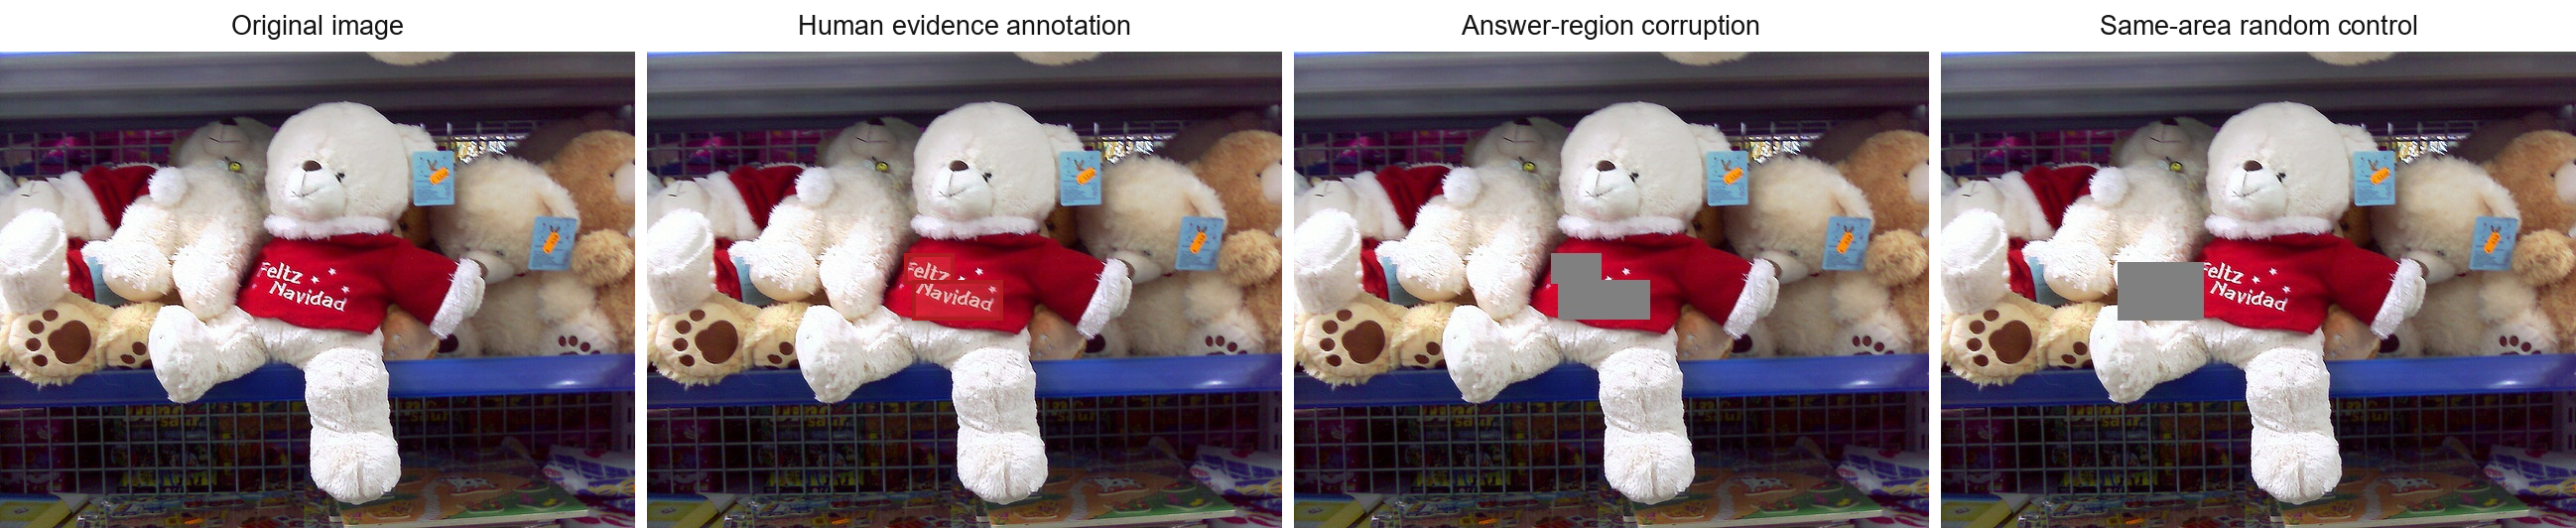
\includegraphics[width=\linewidth,trim=0bp 130bp 1947bp 90bp,clip]{figures/okvqa_val_4739195_input_control_panel.png}
\normalsize (a) Original
\end{minipage}\hfill
\begin{minipage}{0.31\linewidth}
\centering
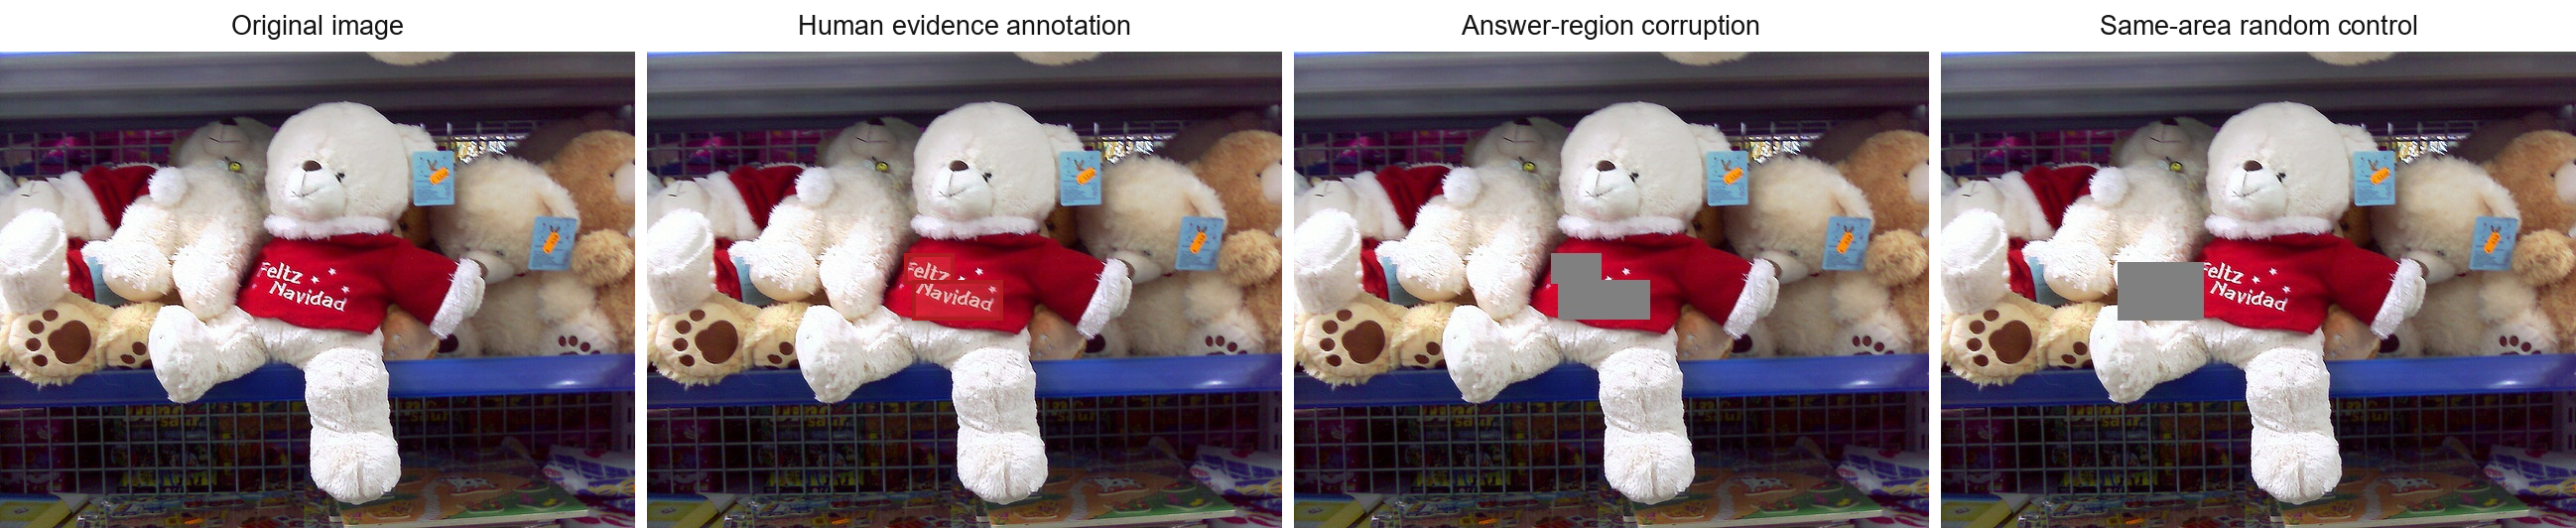
\includegraphics[width=\linewidth,trim=1298bp 130bp 649bp 90bp,clip]{figures/okvqa_val_4739195_input_control_panel.png}
\normalsize (b) Evidence masked
\end{minipage}\hfill
\begin{minipage}{0.31\linewidth}
\centering
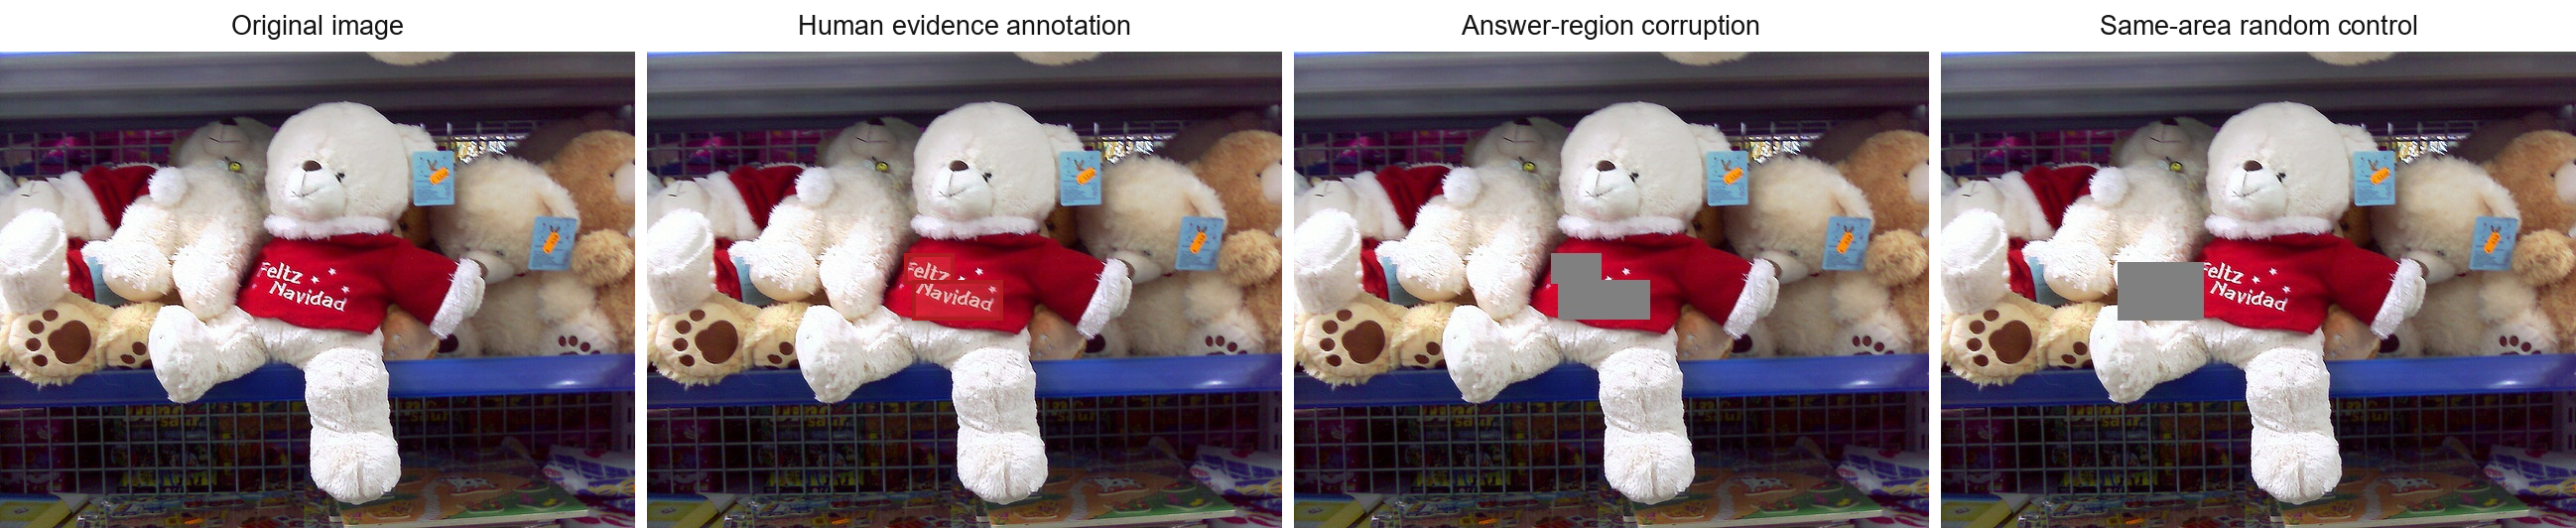
\includegraphics[width=\linewidth,trim=1947bp 130bp 0bp 90bp,clip]{figures/okvqa_val_4739195_input_control_panel.png}
\normalsize (c) Same-area control
\end{minipage}
\caption{\textbf{The matched visual comparison on one compact-evidence question.} For ``What language is the sign on the bear in?'' the target answer is ``Spanish.'' Gray corruption covers the annotated text in (b) and an equally sized non-evidence region in (c). The panels illustrate the paired input conditions, not a single-case mechanism result; the full human annotation is shown in Appendix~\ref{app:annotation-protocol}.}
\label{fig:visual-mask-example-main}
\end{figure}
\FloatBarrier

\subsection{Testing internal objects in both directions}

At a specified layer and position group, let $o$ be the complete dense state or a restricted candidate derived from it. $\mathtt{Restore}(o,c)$ writes the clean value of $o$ into a corrupted run $c$. $\mathtt{Delete}(o,c)$ is shorthand for writing the value recorded under $c$ into the otherwise clean run; it does not zero the object. Their target-score effects are
\begin{align}
B_S(x,a;o,c)&=S(x,a;\mathtt{Restore}(o,c))-S(x,a;c),
\label{eq:restoration-benefit}\\
A_S(x,a;o,c)&=S(x,a;c_0)-S(x,a;\mathtt{Delete}(o,c)).
\label{eq:deletion-damage}
\end{align}
Restoration measures recovered support; corrupted-state replacement measures support lost from the clean run. The two writes use the same paired state difference in opposite baseline runs, so they are complementary intervention tests rather than independent samples. A clean state copied into a damaged run can improve an answer without showing that the state was needed in the clean run; a masked state inserted into a clean run can lower the score without showing that the clean state would rescue a damaged input. We therefore compare both effects with the same natural clean-to-mask score loss. A large intervention effect alone is not enough: recovery far above the natural loss also fails to reproduce it faithfully.

Candidate classes include complete hidden states, a fitted sparse reconstruction and its remaining reconstruction error at the same feed-forward output, selected native feed-forward channels, and a low-rank hidden-state subspace shared across examples within one model. The sparse tool is a separate measurement interface; native channels belong to the base model. References differ: full feed-forward output for sparse reconstruction, all channels for native groups, and the natural clean-to-mask score change for shared subspaces and full hidden states. Each candidate must meet its own reference and control gates in both directions before we call it a complete path. Appendix~\ref{app:detailed-method} gives the feature selection, decoder reconstruction, residual, subspace projection, and intervention details; the next section fixes the evaluation sets and statistical criteria.

\section{Experimental Setup}
\label{sec:experimental-setup}

We evaluate three frozen vision--language models with model-specific sparse measurement tools: Gemma3 and Qwen2.5-VL use per-layer transcoders, and LLaVA1.5 uses a cross-layer transcoder \citep{gemma3,qwen25vl,llava,dunefsky2024transcoders,ameisen2025circuittracing}. The tools are fitted separately from the base models. The regional evaluations draw from compact-evidence questions in the OK-VQA validation split \citep{okvqa}; Appendix~\ref{app:detailed-setup} specifies each evaluation set and its selection rule. Cross-model comparisons align the image--question examples, visual corruption, fixed answer target, intervention direction, and statistical interpretation, not raw feature identities or score magnitudes.

\begin{center}
\begin{minipage}{\linewidth}
\captionsetup{type=table,hypcap=false}
\caption{\textbf{Evaluation roles and independent units.} Dash: no interface selection; 61+52: separate evaluations; 60/61: accepted/reviewed masks.}
\label{tab:evaluation-roles}
\centering
\small
\begin{tabular*}{\linewidth}{@{\extracolsep{\fill}}lccc@{}}
\toprule
Comparison & Selection & Evaluation & Inference unit \\
\midrule
Regional and hidden-position & -- & 61 + 52 & image--question \\
Answer-position, sparse, native & 60 & 240 & 48 clusters \\
Shared-subspace rank & 40 fit + 20 select & 40 & image--question \\
LLaVA full-hidden confirmation & frozen interface & 60 / 61 masks & image--question \\
Matched late-answer diagnostic & rule from LLaVA & same 60 & image--question \\
\bottomrule
\end{tabular*}
\end{minipage}
\end{center}

Table~\ref{tab:evaluation-roles} separates groups that answer different questions. The 61-example expanded set and 52-example set selected without model results test whether regional damage and hidden-position preferences repeat. The 240-image set reuses previously analyzed images to compare internal candidates under stronger intervention controls; it is not a fresh confirmation set. Forty, twenty, and forty disjoint images respectively fit, select, and replicate the shared-subspace candidates. Only the final LLaVA full-hidden test uses newly reviewed evidence masks after freezing its interface and decision rule. The same 60 masks are subsequently reused in a three-model comparison whose relative-layer rule was chosen after the LLaVA finding.

Every paired comparison uses the same fixed short-answer tokenization across clean, evidence-masked, control-masked, and internally intervened runs. The 61- and 52-example regional analyses resample image--question examples; their individual 95\% intervals are unadjusted across panel cells and describe the direction and recurrence of the matched contrasts. The 240-image tests resample 48 entity--relation clusters and jointly correct their comparison families. Shared-subspace and complete hidden-state candidates must restore and remove 80--120\% of the mean clean-minus-evidence-mask sequence-score change. For independent confirmation, we resample image--question examples while keeping each example's clean, masked, and intervened scores together. In each of the two write directions, the 95\% lower bound must be nonnegative both for the candidate effect minus 80\% of the natural loss and for 120\% of that loss minus the candidate effect: four bounds in total. The later three-model result is diagnostic rather than jointly prospective. Appendix~\ref{app:detailed-setup} gives all splits, target rules, reconstruction diagnostics, exact resampling counts, and model-specific layer settings.

\section{Experiments and Results}
\label{sec:experiments-results}

The experiments follow the three evidence levels introduced above. Matched masks establish whether the annotated region contributes more answer support than comparable image content; hidden restoration tests where that support is recoverable; bidirectional interventions compare proposed internal objects with their corresponding complete references. The final LLaVA confirmation directly matches a full-hidden intervention to the natural clean-to-mask score change. Appendix~\ref{app:detailed-results} contains the complete numerical results and controls.

\subsection{Localized evidence changes answers beyond generic image damage}
\label{sec:main-regional}

Figure~\ref{fig:behavior-region-specificity} tests the first level using the complete-answer sequence score. In the expanded 61-example set, Qwen and LLaVA have intervals above zero and Gemma's interval crosses zero; all three intervals lie above zero in the independently selected 52-example set. The first-token rank intervals are above zero for all six model-by-set comparisons (Appendix~\ref{app:detailed-results}). Together, these scores show that the annotated region contributes answer support beyond generic equal-area image damage in this compact-evidence setting.

\begin{figure}[!htbp]
    \centering
    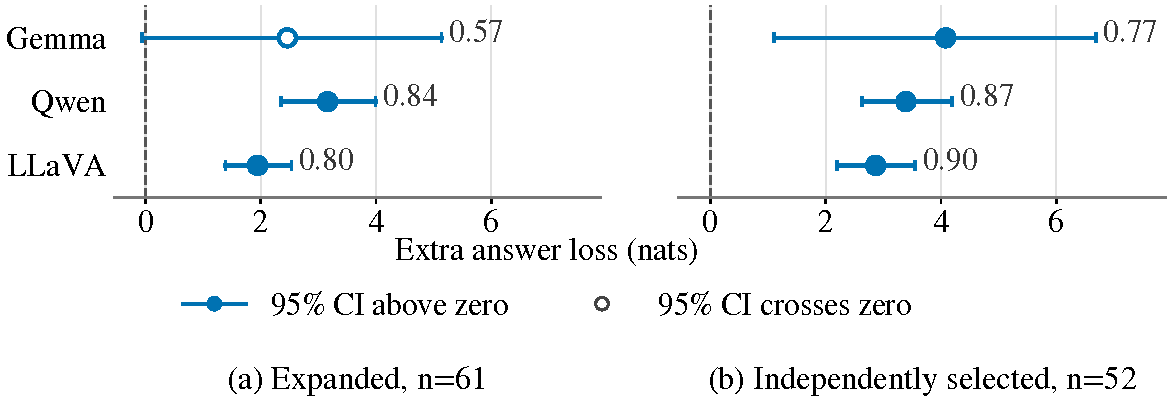
\includegraphics[width=\linewidth]{figures/2026-09-25-main-readable/behavior_region_specificity.pdf}
    \caption{\textbf{Answer-region corruption reduces complete-answer support beyond matched occlusion.} Panels (a) and (b) show separate sets of 61 and 52 compact-evidence examples on a shared raw log-probability scale. Each mark is the mean additional complete-answer score loss from masking the answer region rather than a same-area random region; whiskers are unadjusted 95\% sample-bootstrap intervals. Filled markers have intervals above zero; the hollow marker crosses zero. Numbers give positive-sample fractions. First-token rank results are in Appendix~\ref{app:detailed-results}.}
    \label{fig:behavior-region-specificity}
\end{figure}

\subsection{Clean hidden states recover the evidence-specific loss}
\label{sec:main-hidden}

Figure~\ref{fig:hidden-restoration-specificity} establishes the second level using the raw target-logit score: aligned clean hidden states recover more under answer-region corruption than under same-area random corruption. Gemma and Qwen show positive intervals across pooled visual positions, while LLaVA shows a positive interval at predefined answer-adjacent positions rather than across all visual positions. The first-token rank contrasts support the same position pattern (Table~\ref{tab:main-hidden-rank}). The independently selected 52-example grid retains this pattern. A separate 240-image evaluation freezes answer-position layers on 60 development images, then compares correct restoration with equal-norm random directions, reversed differences, and wrong insertion positions. All 12 jointly corrected differences are positive for the aligned restoration relative to their baselines or controls, connecting the regional score loss to specific internal content, direction, and location (Appendix~\ref{app:detailed-results}).

\par\smallskip
\noindent
\begin{minipage}{\linewidth}
    \captionsetup{type=figure,hypcap=false}
    \centering
    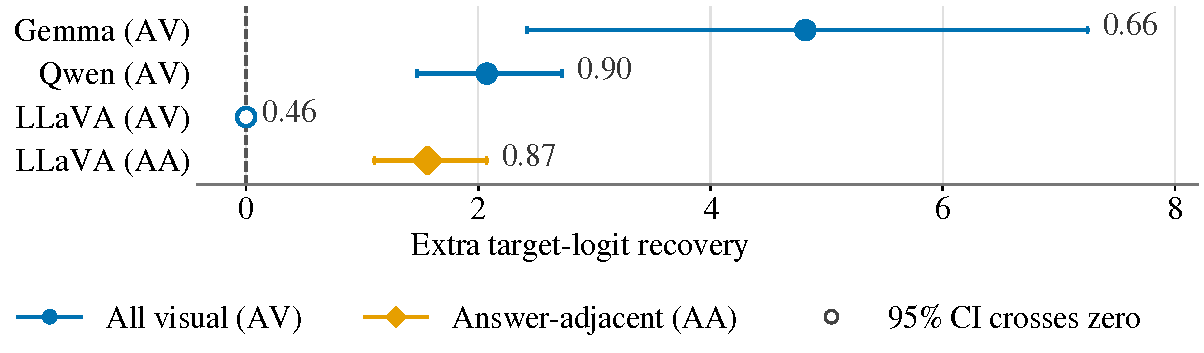
\includegraphics[width=\linewidth]{figures/2026-09-25-main-readable/hidden_restoration.pdf}
    \caption{\textbf{Aligned hidden restoration recovers additional target-logit support under evidence masking.} Raw answer-region-minus-random restoration effects on 61 examples; whiskers are unadjusted 95\% sample-bootstrap intervals. Filled marks lie above zero, the hollow mark crosses zero, and numbers give positive-sample fractions. AV pools visual positions; AA uses four answer-adjacent positions. Rank contrasts appear in Table~\ref{tab:main-hidden-rank}.}
    \label{fig:hidden-restoration-specificity}
\end{minipage}
\par\smallskip

\begin{minipage}{\linewidth}
    \captionsetup{type=table,hypcap=false}
    \caption{\textbf{Rank recovery follows the logit position pattern.} $\Delta s_{\mathrm{rank}}$ is the answer-mask restoration gain minus the same-area-random-mask gain on 61 examples. Brackets are unadjusted 95\% sample-bootstrap intervals; AV pools visual positions, and AA uses four answer-adjacent positions.}
    \label{tab:main-hidden-rank}
    \centering
    \normalsize
    \begin{tabular*}{\linewidth}{@{\extracolsep{\fill}}lrrr@{}}
    \toprule
    Model--position & $\Delta s_{\mathrm{rank}}\uparrow$ & 95\% interval & Positive fraction \\
    \midrule
    Gemma (AV) & 14,444.7 & [7,248.8, 23,404.2] & .738 \\
    Qwen (AV) & 2,711.5 & [549.4, 6,147.1] & .869 \\
    LLaVA (AV) & 1.23 & [-.25, 2.96] & .393 \\
    LLaVA (AA) & 500.2 & [124.9, 1,017.9] & .836 \\
    \bottomrule
    \end{tabular*}
\end{minipage}

\subsection{Effect matching distinguishes internal descriptions}
\label{sec:main-effect-matching}

The third level compares each candidate's two score effects with the complete intervention at its own interface. We first test compact fitted, native-channel, and shared-subspace descriptions, then use a frozen complete hidden state as a positive reference.

\subsubsection{Readable structure does not guarantee effect matching}
\label{sec:main-restricted}

The sparse comparison begins with reconstruction fidelity. On a separate 60-image development set (59 valid images for LLaVA), at 128 selected features the fitted tools have mean relative squared reconstruction errors (residual squared norm divided by full-change squared norm) of 1.76, 1.87, and 1.62 for Gemma, Qwen, and LLaVA, with mean direction similarities of .23, .22, and .20. Each error exceeds one: the squared reconstruction residual is larger than the squared complete change. The fitted tools therefore poorly reconstruct the internal change they are asked to explain (definitions in Appendix~\ref{app:detailed-setup}; per-model counts in Appendix~\ref{app:detailed-results}).

At matched feed-forward outputs on the same 240 evaluation images per model, Figure~\ref{fig:sparse-component-effects} shows no positive effect from the selected sparse reconstruction after correction over 72 tests. Yet the fitted tools' normalized feature summaries differ in 16 of 24 paired comparisons (Appendix Table~\ref{tab:sparse-structure-summary}). Readable structural variation and faithful reconstruction of a controlled answer effect are therefore distinct findings.

\par\smallskip
\noindent
\begin{minipage}{\linewidth}
    \captionsetup{type=figure,hypcap=false}
    \centering
    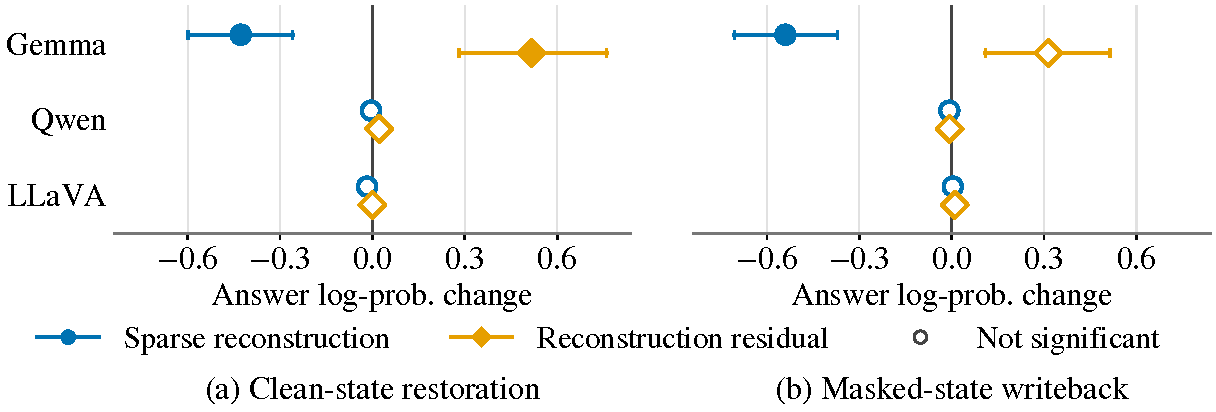
\includegraphics[width=\linewidth]{figures/2026-09-25-main-readable/sparse_component_effects.pdf}
    \caption{\textbf{Selected sparse reconstructions do not yield a reliable positive answer effect.} Panels (a) and (b) show restoration and masked-state writeback at the same feed-forward output on 240 images per model. Whiskers are uncorrected 95\% cluster-bootstrap intervals on a shared raw answer-score scale; filled marks survive the joint 72-test correction. Zero marks no score change.}
    \label{fig:sparse-component-effects}
\end{minipage}
\par\smallskip

Native feed-forward channels remove the fitted-tool reconstruction error and reveal local upstream--downstream links in all three models under positive-only selection. Their score effects, however, over-amplify the full-channel reference: Gemma's selected-group restoration changes the sequence score by 16.47, versus 3.79 for all channels (Appendix Table~\ref{tab:native-channel-path}). The two frozen channel rules select separately for each image using its known answer, and neither meets the full set of effect-matching criteria.

An example-shared linear subspace offers a different compact description. Figure~\ref{fig:main-low-rank-sweep} shows the eight candidate ranks on the 20-image selection set: no rank from 1 to 128 enters the effect-matching band in both directions. Table~\ref{tab:main-rank128} then reports diagnostic rank-128 effects on a separate 40-image set. Retaining hidden-change energy is not sufficient to match the answer effect: restoration can overshoot while masked-state writeback reverses direction. Appendix~\ref{app:detailed-results} reports the full controls and matched late-answer test.

\begin{minipage}{\linewidth}
    \captionsetup{type=figure,hypcap=false}
    \centering
    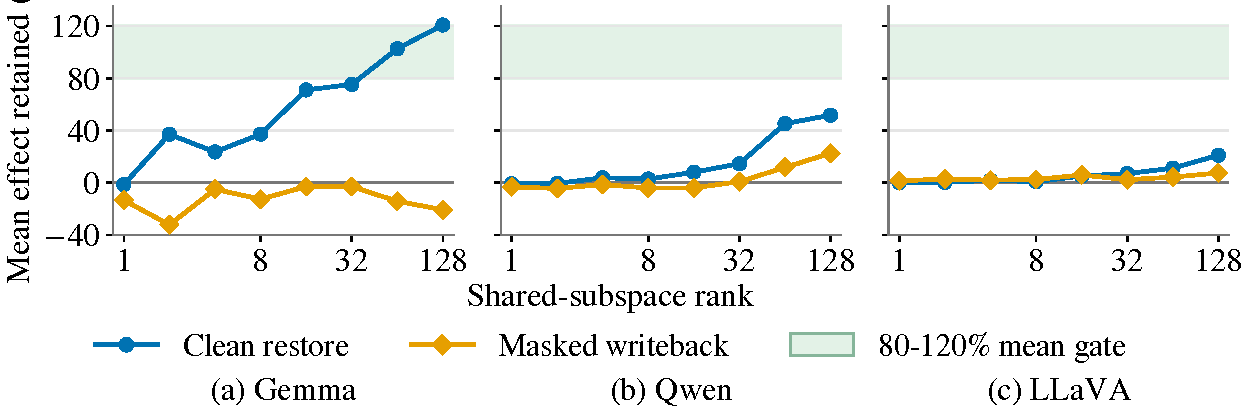
\includegraphics[width=\linewidth]{figures/2026-09-25-main-readable/low_rank_effect_matching.pdf}
    \caption{\textbf{No shared rank matches both directions.} Model-specific bases are fitted on 40 images; curves show restore/writeback effects for ranks 1--128 on a separate 20-image selection set, as percentages of mean natural clean-to-mask score change. Both must enter the shaded 80--120\% band at the same rank; none does.}
    \label{fig:main-low-rank-sweep}
\end{minipage}

\begin{minipage}{\linewidth}
    \captionsetup{type=table,hypcap=false}
    \caption{\textbf{Hidden-change energy does not ensure answer-effect matching.} Diagnostic rank-128 values on 40 separate images. Energy is retained squared hidden-change norm; restore/writeback are percentages of the mean natural score change. No rank passed selection.}
    \label{tab:main-rank128}
    \centering
    \normalsize
    \begin{tabular*}{\linewidth}{@{\extracolsep{\fill}}lrrr@{}}
    \toprule
    Model & Energy (\%) & Restore (\%) & Masked writeback (\%) \\
    \midrule
    Gemma & 88.9 & 425.0 & -357.7 \\
    Qwen & 53.1 & 53.0 & 51.2 \\
    LLaVA & 15.9 & 10.5 & 0.1 \\
    \bottomrule
    \end{tabular*}
\end{minipage}

\subsubsection{A complete LLaVA hidden state matches both directions}
\label{sec:main-full-hidden}

The complete hidden state provides a positive reference for effect matching. At LLaVA layer 30 and four answer-adjacent positions, restoration and masked-state writeback retain 93.0\% and 91.0\% of the mean clean-to-mask score change on the 20-image selection set, then 94.9\% and 92.4\% on a separate 40-image replication set. We freeze that interface before testing 60 accepted evidence masks reviewed without model results. On this independent set, clean-state restoration recovers 95.8\% and masked-state writeback removes 95.0\% of the mean natural clean-to-mask sequence-score change. All four predeclared paired-bootstrap bounds pass (Appendix Table~\ref{tab:llava-hidden-confirmation}); a post-hoc 15--30\% tolerance check gives the same decision (Appendix~\ref{app:gate-tolerance}). The same frozen internal location therefore nearly reproduces the natural score change in both directions.

A later same-sample comparison tests the penultimate language layer and four answer-adjacent positions in all three models. For LLaVA, this rule reuses the confirmed layer and positions under a common three-model run rather than selecting a new interface. At these matched relative locations, LLaVA again passes all four bounds (95.2\% restoration; 95.7\% writeback), Qwen reaches 74.3\% and 45.3\%, and Gemma's mean effects reverse direction. This common-location rule was chosen after the LLaVA confirmation, making the three-model comparison a diagnostic of the specified interfaces. Figure~\ref{fig:bidirectional-full-hidden} places it beside the independently confirmed LLaVA result; Appendix~\ref{app:detailed-results} reports its gate margins and sample-level accounting.

\par\smallskip
\noindent
\begin{minipage}{\linewidth}
    \captionsetup{type=figure,hypcap=false}
    \centering
    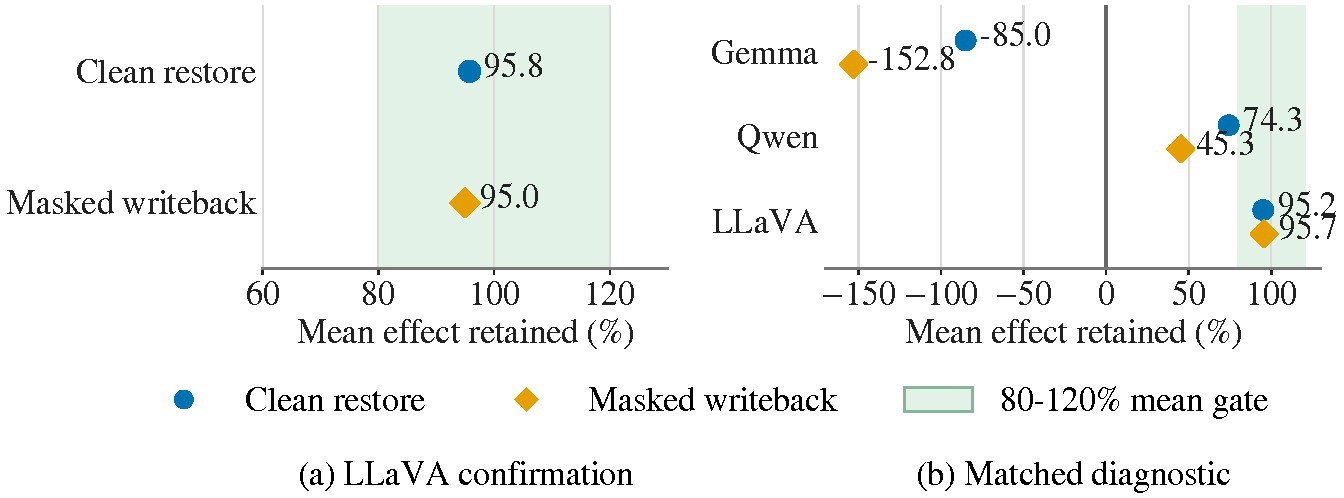
\includegraphics[width=\linewidth]{figures/2026-09-25-main-readable/full_hidden_bidirectional.pdf}
    \caption{\textbf{One independently confirmed complete hidden-state interface; a separate matched diagnostic.} Each mark divides the within-model mean restoration or masked-state-writeback effect by the mean clean-minus-masked sequence-score change. The shaded 80--120\% band is a mean gate, not a confidence interval. Panel (a) confirms the frozen LLaVA interface on 60 accepted masks with all four paired-bootstrap bounds passing. Panel (b) reuses those masks under a relative-layer rule chosen afterward; only the evaluated LLaVA interface passes all four bounds. Negative ratios reverse the mean effect; the panels use independent horizontal scales.}
    \label{fig:bidirectional-full-hidden}
\end{minipage}
\par\smallskip

\FloatBarrier


\section{Discussion}

The region-anchored audit provides a common target for comparing different internal descriptions. Matched corruption shows that changing the annotated region causes additional answer-score loss; aligned hidden restoration locates positions where part of that loss can be recovered. The paired internal writes then ask a stronger question: does a specified object reproduce the effect of the corresponding complete intervention in both directions? The evidence mask defines the visual change under study, while each internal candidate is judged against its own complete reference.

The results make this distinction consequential. The fitted sparse tools display different feature structures across models, yet poorly reconstruct the evidence-induced internal change and do not yield a reliable positive sparse-reconstruction score effect. Native channels reveal local interactions without fitted-tool error, but their selected groups overshoot the complete-channel reference. Shared low-rank projections test a distributed alternative and also miss the bidirectional gate. This \textbf{dependence--visibility gap} separates an evidence-specific answer response from incomplete reproduction by a specified internal description. Its size depends on the tested model--interface pair.

The independently confirmed LLaVA result gives a constructive answer-side example: at one frozen interface, complete hidden states nearly restore the natural score loss when copied into the masked run and remove nearly the same amount when their masked values are written into the clean run. This full-effect reference gives the compact-candidate comparisons a measured target. The resulting audit can compare internal descriptions across models without requiring their feature coordinates to align: measure the visual score change, test both directions of the candidate intervention, and compare with the appropriate complete reference. Appendix~\ref{app:detailed-limitations} details the evaluation scope, interface-specific boundaries, and annotation workflow.

\section{Conclusion}

We introduced a region-anchored audit that measures whether an internal description reproduces the answer-score effect of removing localized visual evidence. Across three vision--language models, annotated-region masks cause more score loss than same-area controls, and aligned hidden-state restoration selectively recovers it. The tested compact descriptions and the frozen LLaVA complete hidden-state interface span markedly different degrees of effect matching; the latter independently restores and removes about 95\% of the natural score change. Bidirectional effect matching therefore provides a common, measurable standard for comparing what different representation lenses explain about visual evidence use.


\clearpage
\section*{AI Use Statement}

Generative AI tools assisted with experimental-design discussions, analysis and figure code, manuscript drafting and editing, and initial pre-annotation of evidence masks. The pre-annotated masks used in the independent LLaVA confirmation were reviewed by a human without access to model results. AI-assisted text, code, and analyses were checked against the recorded data and experimental outputs. The authors take responsibility for the final manuscript and its results.

\section*{Reproducibility Statement}

The evaluated model and sparse-tool interfaces, human evidence masks, fixed answer targets, sample splits, intervention rules, and statistical decision criteria are specified in the Method, Experimental Setup, and Appendices~\ref{app:model-background}--\ref{app:prompt-text}. The appendices preserve the full result tables, reconstruction and projection definitions, mask-review decisions, cluster-resampling procedures, and script and checkpoint identifiers needed to rebuild every reported figure and table. Upon publication, we plan to release the masks, manifests, evaluation code, and figure-source summaries; externally hosted model and sparse-tool weights remain identified by their public names and recorded hashes.


\bibliographystyle{iclr2027_conference}
\bibliography{references}

\clearpage
\appendix

\section{Model computation and sparse-interface background}
\label{app:model-background}

This section introduces the model-side objects needed to state our problem. We first describe how a vision--language model (VLM) produces an answer and what its dense internal state represents. We then introduce sparse transcoders as separate tools for viewing part of the dense internal state. With the base computation and the fitted measurement interface separated, we can state which internal objects may preserve the answer effect of localized visual evidence.

\stitle{VLM computation.}
A VLM receives an image and a question and generates an answer one token at a time. Answer generation is autoregressive: after producing or receiving an answer prefix, the model uses that prefix together with the image and question to predict the next token. We write $x=(I,q)$ for the input image $I$ and question $q$, and $a=(a_1,\ldots,a_T)$ for a fixed target answer containing $T$ tokens. The index $t\in\{1,\ldots,T\}$ identifies one answer token, $a_{<t}$ is the prefix preceding $a_t$, and $\mathcal{V}$ is the set of tokens in the model vocabulary. The frozen parameters of the VLM are denoted by $\theta$.

Before the model predicts $a_t$, it represents the image, question, and answer prefix as one joint sequence of visual and text positions. This sequence passes through $L$ residual-stream layers indexed by $\ell\in\{0,\ldots,L-1\}$. At every position, the residual stream is the running internal vector that carries information from one layer to the next while the layer's attention and feed-forward calculations update it \citep{elhage2021transformerCircuits}. Attention combines information across positions, whereas the feed-forward calculation transforms the vector at each position. Let $n_{\mathrm{pos}}$ be the number of positions in the joint sequence and $d$ the dimension of each residual-stream vector. We write
\begin{equation}
    \vec{h}_{i}^{\ell}(x,a_{<t};\theta)\in\mathbb{R}^{d}
    \label{eq:dense-state}
\end{equation}
for the residual-stream state at position $i\in\{1,\ldots,n_{\mathrm{pos}}\}$ in layer $\ell$. Because this vector retains all $d$ coordinates at that position, we refer to it as a \emph{dense} state.

After the final layer, the model produces a vector $\vec{z}_{t}(x,a_{<t};\theta)\in\mathbb{R}^{|\mathcal{V}|}$. Each entry is the model's score for one possible next token before those scores are converted to probabilities; these entries are called logits. The entry associated with $a_t$ therefore records the model's direct support for the next target token. Repeating this prediction step generates the complete answer.

\stitle{Sparse representations.}
The dense state records the full internal vector at one layer and position, but its individual coordinates do not automatically correspond to separately understandable parts of the computation. A sparse transcoder provides another view. It is trained after the base VLM and kept frozen during analysis, so it is a measurement tool rather than a component that the VLM itself uses to generate the answer. The tool reads a dense state and describes a change that a layer adds to the dense state using a larger set of learned features, while allowing only a small number of those features to be active at once. This limited feature activity is what makes the representation sparse.

Two forms of transcoder are used in this paper. A per-layer transcoder (PLT) uses features to approximate the update produced by the feed-forward calculation within one layer \citep{dunefsky2024transcoders}. A cross-layer transcoder (CLT) reads a feature in one layer and allows that feature to describe contributions written into later layers \citep{ameisen2025circuittracing}. Applying these interfaces to VLM computation follows recent multimodal circuit-tracing work \citep{yang2026vlmcircuittracing}. The distinction matters because a PLT feature has a within-layer target, whereas a CLT feature can have different target layers.

\begin{samepage}
Let $\phi$ denote the frozen parameters of one model-specific sparse interface. In read layer $\ell$, its encoder converts a dense state into a sparse activation vector,
\begin{equation}
    \vec{f}_{i}^{\ell}(x,a_{<t};\theta,\phi)
    =\mathtt{Encode}^{\ell}\!\left(\vec{h}_{i}^{\ell}(x,a_{<t};\theta);\phi\right).
    \label{eq:sparse-encoding}
\end{equation}
This vector lies in $\mathbb{R}^{n_{\mathrm{feat}}^{\ell}}$, where $n_{\mathrm{feat}}^{\ell}$ is the number of available sparse features in layer $\ell$. The index $j\in\{1,\ldots,n_{\mathrm{feat}}^{\ell}\}$ identifies one feature, and its scalar activation is $f_{i,j}^{\ell}=\bigl[\vec{f}_{i}^{\ell}\bigr]_{j}$. Each active feature is paired with a decoder direction that maps its contribution back into the VLM's dense vector space. The Method defines how features are selected, how PLT and CLT decoder directions are indexed by their target layers, and how selected features are reconstructed. A feature index belongs to one fitted interface and does not identify the same internal component in another model or interface.
\end{samepage}

\stitle{Problem definition.}
A \emph{human-localized answer-bearing region} is an image region that an annotator identifies as containing visual information needed for the target answer. Given an image--question input, a target answer, a frozen VLM, and such a region, our first question is whether changing that region alters the model's score for the fixed answer more than changing comparable non-evidence content. Our second question is which internal object retains the answer-relevant internal change caused by the regional perturbation: the complete dense state, the part reconstructed by a fitted sparse interface, selected feed-forward channels that belong to the base model, or a low-dimensional subspace shared across examples.

These questions are related but not equivalent. Showing that changing the complete dense state changes the target-answer score does not show that a sparse reconstruction, a channel group, or a shared low-dimensional projection reproduces the same score change. Likewise, observing different sparse patterns across models does not by itself show that the underlying models use different complete mechanisms, because each restricted object may retain a different part of the dense computation. The next section defines the intervention protocol used to separate these questions.

\section{Detailed scoring and intervention construction}
\label{app:detailed-method}

Our method compares how different vision--language models (VLMs) use localized visual evidence without assuming that their internal coordinates or sparse features are homologous. For each internal-object comparison, we hold the image--question input, evidence corruption, target answer, and answer readout fixed, then vary the object intervened on. This common input-side reference lets us evaluate dense states, fitted sparse reconstructions, native channel groups, and model-specific residual-state subspaces shared across examples without equating their coordinates or claiming that every object is tested on one identical dataset.

The method tests two hypotheses. The \textbf{regional-specificity hypothesis} predicts that corrupting a human-annotated answer-bearing region lowers the target-answer score more than matched non-evidence corruption, and that restoring aligned clean internal states recovers more score under evidence corruption than under matched control corruption. The \textbf{path-preservation hypothesis} asks whether a qualifying internal object can recover the score change caused by masking the evidence and remove a corresponding change when its corrupted value replaces the clean value. Compact sparse, native-channel, and shared-subspace candidates are tested before the complete dense state. Structural differences alone do not satisfy either requirement. This section first defines answer scores and matched causal contrasts, then the internal objects and intervention operations used to test the two hypotheses. Section~\ref{sec:experimental-setup} subsequently fixes the models, evaluation sets, selection roles, and statistical criteria.

\subsection{Evaluation conditions and answer support}

Our comparisons evaluate the same input $x$ and target answer $a$ under different complete forward-run configurations. Let $\mathcal{C}$ be the set of these evaluation conditions. Each $c\in\mathcal{C}$ specifies whether the image is unchanged or corrupted and whether selected internal states are unchanged or intervened on; it is an evaluation configuration rather than an additional text input. To score the same answer in every condition, we provide the fixed target prefix $a_{<t}$ before predicting each token rather than feeding back a condition-specific generated prefix. This teacher-forced forward pass produces condition-specific states $\vec{h}_{i}^{\ell}(x,c;\theta)$ and next-token logit vectors $\vec{z}_{t}(x,c;\theta)$. The target answer and its tokenization remain fixed across paired conditions, so the prefix is omitted from these condition-specific argument lists.

The probability assigned to target token $a_t$ under condition $c$ is
\begin{equation}
    p_t^{c}
    =\frac{\exp\!\left([\vec{z}_{t}(x,c;\theta)]_{a_t}\right)}
           {\sum_{v\in\mathcal{V}}\exp\!\left([\vec{z}_{t}(x,c;\theta)]_{v}\right)},
    \label{eq:target-token-probability}
\end{equation}
where $v$ indexes the tokens in $\mathcal{V}$. We use the answer-support set $\mathcal{S}=\{S_{\mathrm{logit}},S_{\mathrm{seq}},S_{\mathrm{rank}}\}$. The first-token logit score is
\begin{equation}
    S_{\mathrm{logit}}(x,a;c)
    =[\vec{z}_{1}(x,c;\theta)]_{a_1},
    \label{eq:logit-score}
\end{equation}
the complete-answer sequence score is
\begin{equation}
    S_{\mathrm{seq}}(x,a;c)
    =\sum_{t=1}^{T}\log p_t^{c},
    \label{eq:app-sequence-score}
\end{equation}
\begin{samepage}
The first-token rank score is
\begin{equation}
    S_{\mathrm{rank}}(x,a;c)
    =-\mathtt{Rank}\!\left(a_1,\vec{z}_{1}(x,c;\theta),\mathcal{V}\right).
    \label{eq:rank-score}
\end{equation}
The operation $\mathtt{Rank}$ returns the one-based descending rank of $a_1$ among the tokens in $\mathcal{V}$. The negative sign gives all three scores the same direction: larger values mean stronger support for the target answer. For a matched wrong answer $\bar{a}$ to the same input, the correct-versus-wrong margin is
\begin{equation}
    M_S(x,a,\bar{a};c)
    =S(x,a;c)-S(x,\bar{a};c),
    \qquad S\in\mathcal{S}.
    \label{eq:answer-margin}
\end{equation}
A positive margin means that the model assigns greater support to the correct target $a$ than to the matched wrong answer $\bar{a}$.
\end{samepage}

\subsection{Matched causal contrasts}

Let $c_0\in\mathcal{C}$ be the clean condition, $c_{\mathrm{evid}}\in\mathcal{C}$ an evidence-region corruption, and $c_{\mathrm{ctrl}}\in\mathcal{C}$ a matched control corruption. For any answer-support function $S\in\mathcal{S}$ defined above, the damage caused by condition $c$ is
\begin{equation}
    D_S(x,a;c)=S(x,a;c_0)-S(x,a;c).
    \label{eq:app-corruption-damage}
\end{equation}
Larger $D_S$ means that the corruption removes more support for the fixed target answer $a$. The evidence-specific regional contrast is
\begin{equation}
    E_S(x,a;c_{\mathrm{evid}},c_{\mathrm{ctrl}})
    =D_S(x,a;c_{\mathrm{evid}})-D_S(x,a;c_{\mathrm{ctrl}}).
    \label{eq:app-evidence-control-contrast}
\end{equation}
Thus, $E_S>0$ means that corrupting the annotated evidence is more consequential than corrupting its matched control. The clean-to-evidence-mask damage $D_S(x,a;c_{\mathrm{evid}})$ is a different quantity: $E_S$ subtracts the damage from the control mask.

We next connect this input-side deficit to an internal model state. Let $\mathcal{O}$ be the set of intervention objects, where an object $o\in\mathcal{O}$ can be a complete hidden state, a projected hidden-state difference, a selected sparse reconstruction, a reconstruction residual, or a native-channel group. The condition $\mathtt{Restore}(o,c)$ replaces object $o$ in corrupted run $c$ with its clean value. Its restoration benefit is
\begin{equation}
    B_S(x,a;o,c)
    =S\!\left(x,a;\mathtt{Restore}(o,c)\right)-S(x,a;c).
    \label{eq:app-restoration-benefit}
\end{equation}
Restoration tests whether the selected object is sufficient to recover the target-answer score lost under corruption. The complementary condition $\mathtt{Delete}(o,c)$ is shorthand for corrupted-state replacement: it writes the object's value from corrupted run $c$ into the clean run $c_0$, rather than zeroing the object. The resulting deletion damage is
\begin{equation}
    A_S(x,a;o,c)
    =S(x,a;c_0)-S\!\left(x,a;\mathtt{Delete}(o,c)\right).
    \label{eq:app-deletion-damage}
\end{equation}
Deletion damage measures whether replacing the selected object's clean value with its corrupted value removes the clean-versus-corrupted target-score difference. This is a test of necessity under the specified corrupted-state replacement, not under every possible ablation. The comparisons specific to each result evaluate $B_S$ and $A_S$ against equal-norm random directions, reversed clean-state differences, wrong insertion positions, or full-channel references. Together, $E_S$ and these internal controls separate evidence-specific input damage from score changes produced by restoring or replacing one internal object. Restoration alone does not test whether the clean run needs that object's clean value; corrupted-state replacement alone does not test whether restoring it recovers the masked deficit. An object passes the bidirectional interface criterion only if both directions meet their respective gates.

\subsection{Dense and sparse representation changes}

Applying Equation~\ref{eq:sparse-encoding} to a condition-specific dense state defines $f_{i,j}^{\ell}(x,c;\theta,\phi)$. Let $\vec{u}_{i}^{m}(x,c;\theta)\in\mathbb{R}^{d}$ be the complete feed-forward output written at position $i$ in target layer $m$. For a visually corrupted condition $c$, the prefix $\Delta$ denotes a clean-minus-corrupted difference at the same internal object and position:
\begin{align}
    \Delta\vec{h}_{i}^{\ell}(x,c;\theta)
    &=\vec{h}_{i}^{\ell}(x,c_0;\theta)-\vec{h}_{i}^{\ell}(x,c;\theta),
    \label{eq:hidden-difference}\\
    \Delta\vec{u}_{i}^{m}(x,c;\theta)
    &=\vec{u}_{i}^{m}(x,c_0;\theta)-\vec{u}_{i}^{m}(x,c;\theta),
    \label{eq:feedforward-difference}
\end{align}
The first quantity is the residual-state change used for hidden restoration. The second is the complete feed-forward-output change used for the same-object sparse comparison.

Let $\mathcal{J}^{\ell}=\{1,\ldots,n_{\mathrm{feat}}^{\ell}\}$ be the complete feature-index set in read layer $\ell$. For a fixed budget $K$, let $\mathcal{K}_{i}^{\ell}(x,c;K)\subseteq\mathcal{J}^{\ell}$ be the indices of the $K$ largest nonnegative feature activations at position $i$ under condition $c$. The clean and corrupted runs select their top-$K$ indices separately. For feature $j$ read in layer $\ell$, let $\vec{w}_{j}^{\ell\rightarrow m}(\phi)\in\mathbb{R}^{d}$ be its decoder direction into target layer $m\in\{\ell,\ldots,L-1\}$. A PLT uses the within-layer case $m=\ell$; a CLT can write to a later target layer $m>\ell$. The selected-feature reconstruction of the clean--corrupted change at position $i$ is
\begin{equation}
\begin{aligned}
    \widehat{\Delta\vec{u}}_{K,i}^{\ell\rightarrow m}(x,c;\theta,\phi)
    ={}&\sum_{j\in\mathcal{K}_{i}^{\ell}(x,c_0;K)}
      f_{i,j}^{\ell}(x,c_0;\theta,\phi)\,\vec{w}_{j}^{\ell\rightarrow m}(\phi)\\
    &-\sum_{j\in\mathcal{K}_{i}^{\ell}(x,c;K)}
      f_{i,j}^{\ell}(x,c;\theta,\phi)\,\vec{w}_{j}^{\ell\rightarrow m}(\phi).
\end{aligned}
    \label{eq:sparse-reconstruction}
\end{equation}
The hat marks a reconstruction rather than a native model state. Any condition-independent affine decoder offset cancels in this difference. The corresponding reconstruction residual is
\begin{equation}
    \vec{r}_{\mathrm{err},i}^{m}(x,c;\theta,\phi)
    =\Delta\vec{u}_{i}^{m}(x,c;\theta)
     -\widehat{\Delta\vec{u}}_{K,i}^{\ell\rightarrow m}(x,c;\theta,\phi).
    \label{eq:reconstruction-residual}
\end{equation}
The subscript $\mathrm{err}$ identifies a reconstruction residual, not a second causal mechanism. Because the full change, selected reconstruction, and residual are inserted in separate nonlinear forward passes, their answer effects are not assumed to add.

\subsection{Shared residual-state subspaces}

Sparse reconstructions and native channels use particular fitted or axis-aligned coordinates. To test whether the clean-minus-masked hidden-state change is distributed across coordinates but lies in a low-dimensional space shared across examples within one model, we fit a separate orthonormal basis for each model. For a frozen layer $\ell$ and position group, let $\vec{B}_{r}^{\ell}\in\mathbb{R}^{d\times r}$ contain the first $r$ orthonormal directions obtained by uncentered principal-component analysis of the clean-minus-masked differences from a designated fitting split. Section~\ref{sec:experimental-setup} fixes the fitting, selection, and replication roles. For fixed $(x,c;\theta)$, the projection of Equation~\ref{eq:hidden-difference} onto this basis is
\begin{equation}
    \Delta\vec{h}_{r,i}^{\ell}
    =\vec{B}_{r}^{\ell}(\vec{B}_{r}^{\ell})^{\mathsf{T}}
      \Delta\vec{h}_{i}^{\ell}.
    \label{eq:shared-subspace-projection}
\end{equation}
The subscript $r$ is the number of shared basis directions, and $i$ ranges over the frozen position group. Restoration adds $\Delta\vec{h}_{r,i}^{\ell}$ to the masked run, whereas deletion subtracts it from the clean run. The full-hidden reference uses the unprojected $\Delta\vec{h}_{i}^{\ell}$ at the same layer and positions. The fitted basis is an analysis object constructed from intervention differences; it is not a native variable used by the VLM during generation.

\subsection{Common intervention design}

The primary visual treatment is corruption of the human-annotated \emph{answer mask}, which covers the localized region supporting the short answer. When answer-bearing evidence and necessary adjacent context are separately annotated, their union provides a broader evidence condition. The primary control is a same-area random mask on the same image. Gray masking is the common corruption operator; shifted, shuffled, blurred, inpainted, patch-shuffled, dilated, and eroded variants are auxiliary checks reported in the appendix. Ambiguous or diffuse evidence is excluded rather than forced into a compact mask.

Internal interventions evaluate five distinct object classes. \emph{Hidden-state interventions} restore or delete complete residual-stream states at predefined layers and token-position groups. \emph{Sparse-component interventions} insert or remove a selected sparse reconstruction or its reconstruction residual at one matched feed-forward output. \emph{Native-channel interventions} act on coordinates after the gated feed-forward calculation and before its output projection. \emph{Native-channel path tests} jointly manipulate upstream and downstream channel groups. \emph{Shared-subspace interventions} restore or delete the projected hidden-state difference in Equation~\ref{eq:shared-subspace-projection}. This ordering separates an internally recoverable effect, the part visible to fitted sparse coordinates, compact groups of native coordinates, and a compact non-axis-aligned alternative before testing the complete hidden state.

Each result subsection specifies the locations and internal objects needed for its question. Hidden-state locations are compared through a predefined position grid in Section~\ref{sec:shared-dependence}. Sparse components are tested at a matched feed-forward output in Section~\ref{sec:sparse-effect}; Section~\ref{sec:sparse-structure} then describes their normalized structures without treating them as faithful paths. Section~\ref{sec:native-path} tests native-channel candidates without fitted-tool reconstruction error. Section~\ref{sec:subspace-bottleneck} evaluates shared subspaces and the frozen LLaVA full-hidden candidate, ending the intervention sequence with the independent full-hidden confirmation and matched follow-up.

The next section fixes the model--interface pairs, evaluation sets, target construction, selection roles, and statistical criteria before any result is interpreted.

\section{Detailed evaluation setup and statistical criteria}
\label{app:detailed-setup}

The Method defines the common answer scores, intervention objects, and restoration--deletion operations. This section fixes the model--interface pairs, evaluation examples, selection and confirmation roles, answer targets, reconstruction diagnostics, and statistical criteria used to apply those operations. The order matters: we first specify what is compared and which data may select a configuration, then define the diagnostics and uncertainty calculations applied without changing that configuration.

\subsection{Models and evaluation sets}

The protocol is instantiated in three frozen model--lens pairs. \textbf{\modelgemma{}} combines Gemma3 \citep{gemma3} with a per-layer transcoder (PLT), \textbf{\modelqwen{}} combines Qwen2.5-VL \citep{qwen25vl} with a PLT, and \textbf{\modelllava{}} combines LLaVA1.5 \citep{llava} with a cross-layer transcoder (CLT). These names describe our measurement setups, not official variants of the base models. Because the sparse interfaces are model-specific, cross-model tests align the image--question example, corruption, answer readout, intervention direction, and statistical orientation; they do not compare raw feature identities or raw score magnitudes. Native-channel experiments use coordinates from the frozen base models and do not use the transcoders.

We use three groups of evidence-region examples for different experimental roles. The first contains filtered OK-VQA validation examples \citep{okvqa} whose short answer can be determined from a localizable image region. Every example contains an image, a question, a fixed target answer, and a human-annotated evidence mask. The expanded evaluation contains 61 image--question examples. A separate 52-example evaluation is selected and annotated without using model results and serves as the independently selected confirmation for the behavior and hidden-position comparisons. Appendix~\ref{app:annotation-protocol} reports the sample accounting and annotation protocol for these compact-evidence sets.

The answer-position, same-object sparse, native-channel, and descriptive sparse-structure experiments use a second 300-image evidence set. Sixty images select layers, feature budgets, or channel fractions; the remaining 240 images evaluate those frozen choices. The same 240 image identifiers are used for all three models. They belong to 48 predefined groups of related entity--relation questions, which are resampled as clusters rather than treating every image--question row as independent. Because these images appeared in earlier project analyses, we call this a reused confirmation set rather than previously unseen held-out data. Its primary readout is the total log probability of every token in the fixed correct answer.

The third group supports the shared-subspace and full-hidden tests through three disjoint roles. Forty images fit each model's basis, 20 different images select the smallest candidate rank that meets the restoration and corrupted-state-replacement mean gates, and a separate 40-image set is reserved for replication of a selected rank. The tested ranks are $\mathcal{R}=\{1,2,4,8,16,32,64,128\}$, whose elements specify the number of retained basis directions. Earlier hidden-state screening fixed the layer and position group for each model before this subspace analysis: layer 1 at visual positions for Gemma, layer 14 at visual positions for Qwen, and layer 30 at the four answer-adjacent positions for LLaVA. The full-hidden reference is evaluated at the same interfaces. Any full-hidden interface whose mean effects meet the gate in both selection and replication is frozen for final confirmation on a separate pool of 61 candidate masks. Human review is completed without access to model predictions or intervention results, and only accepted masks enter the final confirmation.

A follow-up matched-interface analysis addresses the initial position asymmetry. On the same 60 accepted masks, all three models receive the same intervention at their zero-based penultimate language layer and four answer-adjacent positions: Gemma layer 32 of 34, Qwen layer 26 of 28, and LLaVA layer 30 of 32. The models use the same code, PyTorch runtime, answer-sequence scoring rule, and four paired gates. The shared-subspace test is also repeated at these matched relative locations on the same 40/20/40 fitting, selection, and replication image IDs. This relative-layer rule was chosen after the LLaVA result was known, so the follow-up is a matched diagnostic rather than a jointly prospective confirmation. Model architecture and tokenization remain different.

Answer targets are fixed before each paired comparison. Allowed short-answer aliases come from dataset answers and annotation metadata; once an alias is selected for an example, its tokenization is held constant across the paired corruptions and interventions. Empty targets, formatting failures, and cross-condition token mismatches are excluded from primary estimates and retained in the evaluation accounting. Sequence scores and correct-versus-wrong margins complement the first-token scores when an answer spans multiple tokens or has plausible alternatives.

\subsection{Sparse reconstruction diagnostics}

The same-object experiment first checks how accurately each sparse tool reconstructs the complete clean-minus-corrupted feed-forward-output change. We evaluate this reconstruction on the 60 development images at the four text positions immediately preceding the answer. Let $\mathcal{P}_{\mathrm{ans}}$ be this four-position set and $\mathcal{P}_{\mathrm{nz}}\subseteq\mathcal{P}_{\mathrm{ans}}$ the positions whose complete change is nonzero. The relative squared reconstruction error and mean direction similarity are
\begin{align}
R_{\mathrm{recon}}(x,c)
&=\frac{\sum_{i\in\mathcal{P}_{\mathrm{ans}}}\|\vec{r}_{\mathrm{err},i}^{m}(x,c;\theta,\phi)\|_2^2}
        {\sum_{i\in\mathcal{P}_{\mathrm{ans}}}\|\Delta\vec{u}_{i}^{m}(x,c;\theta)\|_2^2},
\label{eq:relative-reconstruction-error}\\
C_{\mathrm{dir}}(x,c)
&=\frac{1}{|\mathcal{P}_{\mathrm{nz}}|}
  \sum_{i\in\mathcal{P}_{\mathrm{nz}}}
  \frac{\left\langle\widehat{\Delta\vec{u}}_{K,i}^{\ell\rightarrow m},
  \Delta\vec{u}_{i}^{m}\right\rangle}
  {\left\|\widehat{\Delta\vec{u}}_{K,i}^{\ell\rightarrow m}\right\|_2
   \left\|\Delta\vec{u}_{i}^{m}\right\|_2}.
\label{eq:reconstruction-direction-similarity}
\end{align}
The cosine uses the same $(x,c;\theta,\phi)$ arguments as the reconstruction in Equation~\ref{eq:sparse-reconstruction}; these repeated arguments are omitted inside Equation~\ref{eq:reconstruction-direction-similarity} for readability. A zero-norm reconstruction contributes zero similarity, while an image with no complete change at any of the four positions is excluded from the image-level mean. We first compute each scalar within an image and then average across valid development images. A value $R_{\mathrm{recon}}>1$ means that the squared reconstruction error exceeds the squared size of the complete change, while larger $C_{\mathrm{dir}}$ means closer directional agreement.

\subsection{Statistical inference and decision criteria}

The image--question example is the inferential unit. Multiple prompt, mask, feature, or intervention rows belonging to the same example are first averaged within that example; 95\% bootstrap confidence intervals then resample image--question examples rather than raw rows. We report raw row counts only as computational coverage. The 61- and 52-example panel intervals are unadjusted across cells: an interval above zero describes a positive individual contrast, not a family-wise decision. A positive estimate whose interval crosses zero is reported as directional.

For the 240-image experiments, resampling and sign-flip tests operate on the 48 entity--relation clusters. Confidence intervals use 10,000 paired cluster-bootstrap draws and tests use 100,000 sign flips. The answer-position family corrects 12 comparisons together. The sparse-interface family jointly corrects 72 two-sided tests: 36 component effects (three models, three position groups, two components, two directions), 12 random- or wrong-position contrasts (three models, two controls, two directions), and 24 cross-model structural contrasts (three model pairs, two position groups, four summaries). The three component-effect groups are visual positions, answer-adjacent text positions, and their combined set; Figure~\ref{fig:sparse-component-effects} plots only the combined group. This single Holm correction spans effect, control, and structural questions; the 16-, 32-, and 64-feature budget curves are descriptive and are not part of the 72 tests. The native-channel family corrects 66 tests: three models times nine contrasts under positive-only selection and 13 under positive-and-negative selection. A contrast passes only when it meets its predeclared direction or two-sided condition after the corresponding joint correction.

The shared-subspace test uses the complete-answer sequence score and image--question examples as the inferential unit. For a candidate rank, both the mean restoration and mean corrupted-state-replacement effect must fall between 80\% and 120\% of the mean clean-minus-masked sequence-score change on the 20-image selection set. This reference is the clean-to-evidence-mask damage in Equation~\ref{eq:corruption-damage}, not the evidence-versus-control contrast in Equation~\ref{eq:evidence-control-contrast}. Only the smallest passing rank advances to the 40-image replication set, where four paired sample-bootstrap contrasts test the lower and upper bounds for the two directions. A rank that fails selection does not receive strict confirmation. The full-hidden reference uses the same mean gate to nominate one frozen interface. Its independent confirmation requires the 95\% sample-bootstrap lower bounds of all four contrasts to be nonnegative; the mask review, interface, and decision rule are frozen before model evaluation. The matched follow-up applies these four bounds to each model's 60 rows without using its results to rescan layers or positions.

Cross-model conclusions compare score-change direction, positive-sample fraction, within-model retention, and gate status. Raw score changes are not ranked across models because architectures, vocabularies, layers, and intervention coordinates differ. Appendix~\ref{app:sparse-lens-details} records lens checkpoints, layers, and feature counts; Appendix~\ref{app:shared-subspace-details} reports the complete rank sweep and confirmation accounting; and Appendix~\ref{app:detailed-method} defines the intervention procedure.

\section{Detailed intervention results and numerical tables}
\label{app:detailed-results}

This appendix retains the full numerical comparisons behind the three main-text findings. It reports the region-specific behavior and hidden-position grids, the same-object sparse effects and descriptive summaries, native-channel path tests, and the shared-subspace and complete-state comparisons. The main text states the scientific result of each contrast; the tables here preserve all means, intervals, controls, and selection boundaries.

\subsection{Localized visual evidence has region-specific answer effects in all three models}
\label{sec:shared-dependence}

The first question is whether removing the annotated answer region lowers target-answer scores more than removing a comparable non-evidence region in all three models. A second requirement connects that regional loss to internal computation: restoring the aligned clean hidden state must recover more score under answer-region corruption than under matched random corruption. The first comparison establishes regional specificity, the second connects the regional loss to an internal state, and a frozen control set tests whether the recovered content, direction, and location are specific.

\subsubsection{The annotated region matters beyond generic occlusion}

Figure~\ref{fig:behavior-region-specificity} compares answer-region corruption with same-area random corruption on the same image--question examples. Positive values mean that the annotated region causes greater damage to the target rank or complete-answer score. In the expanded 61-example evaluation, the rank intervals lie above zero for all three models, and the complete-answer intervals lie above zero for Qwen and LLaVA; the remaining Gemma interval includes zero. Thus, five of the six model-by-metric estimates lie strictly above zero. In the independently selected 52-example evaluation, both outcomes have intervals above zero in all three models. Removing the annotated answer region therefore causes more damage than removing an equally sized arbitrary region.

\subsubsection{Hidden restoration connects the regional loss to internal computation}

Output damage alone does not show whether the target-score loss can be recovered from an internal model state. We therefore restore clean residual states during the answer-region-corrupted and same-area-random-corrupted runs. For each predefined position group, we compare the restoration benefit under answer-region corruption with that under matched same-area random corruption. The main comparison reports answer-adjacent positions and all visual positions pooled together, so neither position group is selected by improvement in the target answer.

Table~\ref{tab:hidden-position-grid} reports the 61-example comparison. Gemma and Qwen are clearest when all visual positions are restored together, whereas LLaVA is clearest at the predefined answer-adjacent positions. Under those model-specific position groups, both the target-rank and target-logit intervals lie above zero. For LLaVA, the all-visual intervals instead cross zero. Thus, the same region-specific answer-score pattern need not be recovered most strongly at the same type of position in every model.

\begin{center}
\begin{minipage}{\linewidth}
\captionsetup{type=table,hypcap=false}
\centering
\caption{\textbf{Hidden restoration recovers target-answer scores at different position groups.} Entries report the restoration benefit under answer-region corruption minus that under matched same-area random corruption on 61 examples. $\Delta s$ is the mean score change, $\pi$ the positive-sample fraction, and brackets the 95\% sample-bootstrap interval. AV denotes all visual positions pooled together and AA denotes answer-adjacent positions. Rank changes are interpreted within model because vocabulary sizes differ.}
\label{tab:hidden-position-grid}
\normalsize
\begin{tabular*}{\linewidth}{@{\extracolsep{\fill}}lcccc@{}}
\toprule
Model--position & $\Delta s_{\mathrm{rank}}\uparrow$ [95\% CI] & $\pi_{\mathrm{rank}}$ & $\Delta s_{\mathrm{logit}}\uparrow$ [95\% CI] & $\pi_{\mathrm{logit}}$ \\
\midrule
Gemma (AV) & $14{,}444.7\ [7{,}248.8,23{,}404.2]$ & .738 & $4.818\ [2.421,7.249]$ & .656 \\
Qwen (AV) & $2{,}711.5\ [549.4,6{,}147.1]$ & .869 & $2.073\ [1.473,2.722]$ & .902 \\
LLaVA (AV) & $1.23\ [-.25,2.96]$ & .393 & $.001\ [-.005,.007]$ & .459 \\
LLaVA (AA) & $500.2\ [124.9,1{,}017.9]$ & .836 & $1.563\ [1.106,2.072]$ & .869 \\
\bottomrule
\end{tabular*}
\end{minipage}
\end{center}

The independently selected 52-example position grid reproduces the same position-group preference. The mean logit restoration benefit under answer-region corruption exceeds that under same-area-random corruption in all three models, with all-visual positions preferred for Gemma and Qwen and answer-adjacent positions for LLaVA. This replication establishes that the position difference is not specific to the expanded 61-example set.

\subsubsection{Frozen answer-position controls confirm content, direction, and location}

The position-grid result identifies where restoration is clearest, but it does not by itself show that the restored content and direction are specific. We therefore use a separate 60-image development set to choose, for each model, the earliest layer whose mean answer-position restoration reaches at least 90\% of that model's development-set maximum. The selected layers are then frozen and evaluated on the same 240 confirmation images without changing the layer, target answer, four answer-adjacent positions, or control count. Table~\ref{tab:answer-position-confirmation} reports the confirmation results for the restoration itself and the three specificity controls.

\begin{samepage}
\begin{center}
\begin{minipage}{\linewidth}
\captionsetup{type=table,hypcap=false}
\caption{\textbf{Frozen answer-position restoration is specific in all three models.} The Restore column reports the mean increase in complete-answer log probability over the corrupted baseline; the three control columns are paired contrasts between correct restoration and the named intervention, not additional restoration magnitudes. A control contrast can exceed Restore when that control lowers complete-answer log probability below the corrupted baseline. Brackets are 95\% cluster-bootstrap intervals on the same 240 confirmation images. Layers were selected on a separate 60-image development set. All 12 comparisons remain positive after joint correction.}
\label{tab:answer-position-confirmation}
\centering
\small
\setlength{\tabcolsep}{2.4pt}
\begin{tabular*}{\linewidth}{@{\extracolsep{\fill}}lccccc@{}}
\toprule
Model & Layer & Restore & vs. random & vs. reverse & vs. wrong pos. \\
\midrule
Gemma & 28 & \shortstack{$3.956$\\$[2.150,5.781]$} & \shortstack{$3.743$\\$[1.970,5.587]$} & \shortstack{$9.778$\\$[6.960,12.611]$} & \shortstack{$3.135$\\$[1.444,4.924]$} \\
Qwen & 23 & \shortstack{$1.831$\\$[1.086,2.628]$} & \shortstack{$2.108$\\$[1.327,2.949]$} & \shortstack{$5.179$\\$[3.947,6.432]$} & \shortstack{$1.823$\\$[1.082,2.613]$} \\
LLaVA & 20 & \shortstack{$1.060$\\$[0.779,1.359]$} & \shortstack{$1.105$\\$[0.825,1.409]$} & \shortstack{$2.367$\\$[1.833,2.946]$} & \shortstack{$0.987$\\$[0.720,1.274]$} \\
\bottomrule
\end{tabular*}
\end{minipage}
\end{center}
\end{samepage}


Correct restoration is compared with the corrupted baseline, four equal-norm random directions, the reverse of the clean-state difference, and the same difference inserted at the wrong text positions. All four comparisons pass for each model after the 12 tests are corrected together. Randomizing the restored vector, reversing its direction, or inserting it at the wrong positions each reduces the recovery; the consistent reduction ties the restoration gain to the correct internal content, direction, and location. Combined with the regional comparison, the four specificity controls establish the same operational pattern in all three models: answer-region corruption causes greater score loss than matched random corruption, and the aligned clean hidden state selectively recovers that additional loss. The next question is whether a fitted sparse reconstruction preserves the internal change caused by masking the annotated region and produces the corresponding target-score change at its tested feed-forward output.

\FloatBarrier

\subsection{The current sparse tools do not reproduce a positive target-score change}
\label{sec:sparse-effect}

Restoring the complete hidden-state difference increases target-answer scores, but the increase does not show that a fitted sparse reconstruction produces the same score change. We compare complete and sparse interventions at one matched internal object: the feed-forward output at layer 17 for Gemma, layer 14 for Qwen, and layer 16 for LLaVA. For each model, the experiment measures the feed-forward output in the complete-image and answer-region-corrupted runs, reconstructs the output difference with the sparse tool, and writes each candidate difference back at the same position. The combined intervention uses 32 positions sampled uniformly across the visual tokens and the four text positions immediately preceding the answer. Keeping the examples, answer readout, and write locations fixed separates the complete change, sparse reconstruction, and reconstruction residual. We first qualify reconstruction accuracy and then evaluate how inserting or deleting each component changes the complete-answer log probability.

\subsubsection{The sparse tools reconstruct the relevant change poorly}

The fitted sparse tools do not accurately reconstruct the change caused by evidence corruption in the compact-evidence questions studied here. At the primary $K=128$ budget, Equations~\ref{eq:relative-reconstruction-error} and~\ref{eq:reconstruction-direction-similarity} give mean answer-position errors of $1.756$ (Gemma, $n=60$), $1.872$ (Qwen, $n=60$), and $1.617$ (LLaVA, $n=59$), with corresponding direction similarities of $.227$, $.221$, and $.199$. One LLaVA image is excluded from both image-level means because its complete change is zero at all four positions. We therefore interpret the following results as measurements of what each fitted tool reveals, not as direct measurements of a complete sparse mechanism in the base model.

Even under that restricted interpretation, the comparison itself is well controlled. Each model uses the same 240 confirmation images, the same complete-answer log-probability readout, and the same write location for the complete change, sparse reconstruction, and reconstruction residual. At most 128 nonnegative feature activations per token form the main sparse reconstruction; fixed budgets of 16, 32, 64, and 128 are all retained. Original-state writeback, vector decomposition, joint writeback, random-direction norm matching, repeated forward passes, and agreement with the native-channel answer baselines all pass their numerical checks.

\subsubsection{Sparse and remaining components change target-answer scores differently}

Table~\ref{tab:same-object-components} reports the combined visual- and answer-position interventions at the main 128-feature budget. Positive restoration means that inserting a component from the complete-image run increases the correct answer's complete-sequence log probability in the corrupted run. Positive deletion means that removing the corresponding complete--corrupted difference decreases the same sequence score.

\begin{samepage}
\begin{center}
\begin{minipage}{\linewidth}
\captionsetup{type=table,hypcap=false}
\caption{\textbf{The selected sparse reconstruction does not produce a reliable positive target-score change.} Results combine 32 uniformly sampled visual positions with the four text positions immediately preceding the answer and use at most 128 active features per token on the same 240 images per model. Each cell gives the mean change in complete-answer log probability and an uncorrected 95\% cluster-bootstrap interval. Sparse is the selected reconstruction; residual is the reconstruction residual. $\ast$ marks results that remain different from zero after joint correction of 72 tests.}
\label{tab:same-object-components}
\centering
\small
\setlength{\tabcolsep}{2.2pt}
\begin{tabular*}{\linewidth}{@{\extracolsep{\fill}}lcccc@{}}
\toprule
Model & Sparse restore & Residual restore & Sparse delete & Residual delete \\
\midrule
Gemma & \shortstack{$-0.428^{\ast}$\\$[-0.599,-0.260]$} & \shortstack{$0.516^{\ast}$\\$[0.281,0.760]$} & \shortstack{$-0.540^{\ast}$\\$[-0.706,-0.372]$} & \shortstack{$0.314$\\$[0.110,0.515]$} \\
Qwen & \shortstack{$-0.005$\\$[-0.028,0.017]$} & \shortstack{$0.022$\\$[0.002,0.043]$} & \shortstack{$-0.008$\\$[-0.026,0.010]$} & \shortstack{$-0.007$\\$[-0.028,0.012]$} \\
LLaVA & \shortstack{$-0.017$\\$[-0.033,-0.002]$} & \shortstack{$0.000$\\$[-0.017,0.018]$} & \shortstack{$0.003$\\$[-0.008,0.015]$} & \shortstack{$0.010$\\$[-0.006,0.025]$} \\
\bottomrule
\end{tabular*}
\end{minipage}
\end{center}
\end{samepage}


No positive sparse-component score change survives the joint correction in any model. Gemma instead shows negative sparse restoration and deletion changes, while restoring the reconstruction residual increases the sequence score. Qwen and LLaVA show no component-level change after the same correction. The specificity controls reinforce this boundary: no sparse reconstruction outperforms equal-norm random directions or a wrong insertion position, and Gemma's combined-position sparse restoration is significantly weaker than both controls.

The four fixed feature budgets do not reveal a hidden positive pattern. Their mean sparse-restoration changes reverse direction across budgets and remain small for Qwen and LLaVA; Gemma's answer-position change remains negative from 16 through 128 features. These curves are descriptive because the primary joint tests use the frozen 128-feature setting. The conclusion is therefore about the current tools: the tested sparse reconstructions do not produce a reliable positive target-score change under restoration or deletion. This failure does not imply that the base models lack sparse computation, because reconstruction error may prevent the fitted interfaces from reproducing the complete internal change. Before removing the fitted tools from the next causal test, we examine what their sparse descriptions display across models and why those descriptions cannot by themselves establish a path.

\FloatBarrier

\subsection{The sparse tools display different normalized structures across models}
\label{sec:sparse-structure}

The preceding same-object intervention shows that the fitted sparse reconstructions do not reliably recover target-answer scores. Their feature patterns may nevertheless describe how each fitted tool responds to the image corruption. We therefore ask how the clean--corrupted change is distributed within each sparse representation. Because feature identities are not shared across models, we compare normalized summaries rather than raw feature numbers, and we do not use these summaries to infer a faithful path.

\begin{samepage}
The clean--masked support overlap is the fraction of active feature identities shared by the two image conditions. The feature fraction for 80\% of change is the proportion of the tool's full feature set needed to account for 80\% of the squared sparse change; a smaller value means that the change is more concentrated. The positive change-energy fraction measures how much of that squared change comes from features that increase rather than decrease. Finally, the log sparse/full norm ratio compares the size of the sparse reconstruction with the complete internal change within the same model and position group. Table~\ref{tab:sparse-structure-summary} reports these four summaries across models and position groups.
\end{samepage}

\begin{samepage}
\begin{center}
\begin{minipage}{\linewidth}
\captionsetup{type=table,hypcap=false}
\caption{\textbf{The structures seen by the sparse tools differ across models.} Values are model means on the same 240 images. ``Pairs'' counts how many of the three paired model comparisons remain different after the joint correction of 72 tests. These summaries describe each fitted tool and do not align feature identities across models.}
\label{tab:sparse-structure-summary}
\centering
\small
\setlength{\tabcolsep}{2.2pt}
\begin{tabular*}{\linewidth}{@{\extracolsep{\fill}}llrrrr@{}}
\toprule
Summary & Positions & Gemma & Qwen & LLaVA & Pairs \\
\midrule
Clean--masked support overlap & Visual & 0.351 & 0.406 & 0.407 & 2/3 \\
Clean--masked support overlap & Answer & 0.677 & 0.690 & 0.684 & 0/3 \\
Feature fraction for 80\% of change & Visual & 0.0475 & 0.0660 & 0.0345 & 3/3 \\
Feature fraction for 80\% of change & Answer & 0.0142 & 0.0099 & 0.0083 & 3/3 \\
Positive change-energy fraction & Visual & 0.512 & 0.525 & 0.510 & 1/3 \\
Positive change-energy fraction & Answer & 0.491 & 0.495 & 0.519 & 2/3 \\
Log sparse/full norm ratio & Visual & -0.159 & -0.247 & -0.151 & 2/3 \\
Log sparse/full norm ratio & Answer & 0.079 & 0.125 & -0.001 & 3/3 \\
\bottomrule
\end{tabular*}
\end{minipage}
\end{center}
\end{samepage}


Sixteen of the 24 paired model comparisons remain different after all 72 tests are corrected together. The clearest pattern is concentration. At visual positions, the feature fractions needed for 80\% of the change are $.0660$ for Qwen, $.0475$ for Gemma, and $.0345$ for LLaVA; at answer positions, they are $.0142$ for Gemma, $.0099$ for Qwen, and $.0083$ for LLaVA. All six pairwise comparisons for this summary remain different after correction. The other summaries are less uniform: clean--masked support overlap differs for two visual-position pairs but no answer-position pair, while positive change energy differs for one visual-position pair and two answer-position pairs.

These results establish model-conditioned structural differences in what the fitted tools display. They do not establish a shared feature identity, and they do not show that the base models themselves use the same or different complete sparse mechanisms. The earlier intervention found no reliable positive target-score change from these reconstructions despite their different normalized structures. We next remove the fitted tools from the intervention and test whether selected channels belonging to the base models account for the score change.

\FloatBarrier

\subsection{Selected native channels do not form a complete faithful path}
\label{sec:native-path}

The fitted sparse tools show different structures across models, but their small or inconsistent sequence-score changes may reflect the tools rather than the base models. Native channels provide a separate test without fitted reconstruction error. A native channel is one coordinate after the gated feed-forward calculation and before the layer projects that calculation back into the residual stream. It is therefore a pre-projection base-model coordinate, not a coordinate of the residual-space feed-forward output reconstructed in Section~\ref{sec:sparse-effect}. Native channels are not assumed to be individually meaningful features.

The upstream group covers all visual-token positions in the first half of each model's language layers. The downstream group covers the four answer-adjacent text positions in the second half. This split is fixed at half of the language network and is not chosen from answer effects.

On the 60-image development set, each image's known correct answer is used to score and rank its channels. The development results freeze the selection rule and retained fraction, rather than one shared list of channels. One rule retains only channels with the largest positive contributions to the answer. A second rule retains channels with the largest positive or negative contributions, preventing important suppressive contributions from being discarded. The first rule freezes 1\% per layer in all three models; the second freezes 10\% for Gemma, 5\% for Qwen, and 10\% for LLaVA. The same rule and fraction are then applied separately to each confirmation image using that image's known correct answer. The selected confirmation set is therefore answer-conditioned and image-specific. The experiment tests whether such compact per-image support sets satisfy additional path criteria; it does not identify one answer-independent channel set shared across images.

A compact path must satisfy more than a large selected-group sequence-score change. The selected upstream and downstream groups must jointly change the score more than equal-norm random groups; fixing the downstream group in its corrupted state must weaken the upstream restoration; and restoring the downstream group must recover part of an upstream deletion. A faithful path must additionally stay within 80--120\% of the corresponding full-channel score change, preserve the answer after channels outside the selection are removed, and show little recovery from those outside channels alone. Table~\ref{tab:native-channel-path} evaluates both selection rules against these criteria.

\begin{samepage}
\begin{center}
\begin{minipage}{\linewidth}
\captionsetup{type=table,hypcap=false}
\caption{\textbf{Strong native-channel effects do not establish a faithful compact path.} Restore and delete columns report two raw complete-answer log-probability effects separated by a slash: selected channels first, full-channel reference second. The slash does not denote a ratio. Positive-only selection retains 1\% of channels per layer; the second selection retains the largest positive and negative contributions. ``Local link'' requires the upstream blocking and downstream bypass tests to beat matched random groups after the 66-comparison correction. A faithful path additionally requires effect matching and the tests of channels outside the selection.}
\label{tab:native-channel-path}
\centering
\small
\setlength{\tabcolsep}{1.8pt}
\begin{tabular*}{\linewidth}{@{\extracolsep{\fill}}llccccc@{}}
\toprule
Model & Selection & Kept & Restore selected/full & Delete selected/full & Local link & Faithful path \\
\midrule
Gemma & Positive only & 1\% & 16.472/3.791 & 50.084/3.294 & Yes & No \\
Gemma & Positive + negative & 10\% & 3.940/3.791 & 3.237/3.294 & No & No \\
Qwen & Positive only & 1\% & 4.506/1.859 & 12.709/1.706 & Yes & No \\
Qwen & Positive + negative & 5\% & 1.869/1.859 & 1.414/1.706 & Yes & No \\
LLaVA & Positive only & 1\% & 2.972/-0.288 & 7.082/1.935 & Yes & No \\
LLaVA & Positive + negative & 10\% & 0.474/-0.288 & 0.815/1.935 & No & No \\
\bottomrule
\end{tabular*}
\end{minipage}
\end{center}
\end{samepage}


Positive-only selection produces a local upstream--downstream link in all three models, but its effects are not faithful to the full-channel reference. Gemma restoration is $16.472$ compared with a full-channel effect of $3.791$, and its deletion effect is $50.084$ compared with $3.294$. Qwen and LLaVA show the same over-amplification pattern. Selecting both positive and negative contributions brings the Gemma and Qwen restoration means close to their full-channel references, but the full set of criteria still fails.

The positive-only local links survive the 66-comparison correction in all three models, but their strong over-amplification fails full-channel effect matching. Under the positive-and-negative rule, only Qwen shows an answer-conditioned local upstream--downstream link: its blocking and bypass advantages over matched random groups have corrected $p$-values of $.0138$ and $.0438$. Qwen still does not pass the complete effect-matching and outside-channel tests. Gemma does not show a specific downstream handoff under this rule, and LLaVA's full-channel restoration reference is itself negative and uncertain. No model therefore provides a complete, faithful native-channel path under either frozen rule.

The native-channel test removes the fitted sparse tool from the intervention, yet no selected channel group forms a complete faithful path. This rules out the tested axis-aligned groups, not a distributed combination of channels. The remaining compact alternative is therefore a non-axis-aligned subspace shared across examples. The next section tests that alternative before returning to the complete hidden-state change.

\FloatBarrier

\subsection{Shared low-rank candidates fail; one LLaVA full-hidden interface passes}
\label{sec:subspace-bottleneck}

The sparse and native-channel tests leave a specific alternative unresolved. The clean-minus-masked hidden-state change may be distributed across individual coordinates while remaining confined to a low-dimensional residual-state subspace shared across examples within each model. We test this possibility before interpreting the complete hidden-state intervention. The experiment fits a separate basis for each model at frozen interfaces: layer 1 at visual positions for Gemma, layer 14 at visual positions for Qwen, and layer 30 at the four answer-adjacent positions for LLaVA.

\subsubsection{No example-shared rank from 1 to 128 passes the bidirectional gate}

For each model, 40 images fit the uncentered basis in Equation~\ref{eq:shared-subspace-projection}; 20 different images select among ranks $1,2,4,8,16,32,64,$ and $128$; and a separate 40-image set is reserved for replication. A candidate must restore and remove between 80\% and 120\% of the mean clean-minus-masked sequence-score change on the selection images. No tested rank passes both mean gates in any model, so no rank advances to strict confirmation. Table~\ref{tab:shared-subspace-summary} reports the largest tested rank on the replication images together with the full-hidden reference at the same interface.

\begin{samepage}
\begin{center}
\begin{minipage}{\linewidth}
\captionsetup{type=table,hypcap=false}
\caption{\textbf{An example-shared 128-dimensional subspace fails bidirectional effect matching at the initial interfaces.} Gemma/Qwen use visual positions and LLaVA uses answer-adjacent positions, each at its initially selected layer. Values are percentages of the mean clean-minus-masked sequence-score change on the separate 40-example replication set. Energy is the squared hidden-difference norm retained by the projection. Values above 100 indicate effect overshoot, and negative values indicate effect reversal. Rank 128 is the largest tested subspace; no rank from 1 to 128 passes both restoration and corrupted-state-replacement selection gates in any model. Full columns report the unprojected hidden-state reference at the same layer and positions.}
\label{tab:shared-subspace-summary}
\centering
\normalsize
\setlength{\tabcolsep}{2.8pt}
\begin{tabular*}{\linewidth}{@{\extracolsep{\fill}}lrrrrr@{}}
\toprule
Model & Rank-128 energy & Rank-128 restore & Rank-128 delete & Full restore & Full delete \\
\midrule
Gemma & 88.9 & 425.0 & -357.7 & 192.3 & 83.2 \\
Qwen & 53.1 & 53.0 & 51.2 & 94.6 & 76.5 \\
LLaVA & 15.9 & 10.5 & 0.1 & 94.9 & 92.4 \\
\bottomrule
\end{tabular*}
\end{minipage}
\end{center}
\end{samepage}


Retaining substantial hidden-difference energy is not sufficient for causal fidelity. Gemma's rank-128 projection retains 88.9\% of the squared difference but over-restores the answer effect and reverses the deletion effect. Qwen retains 53.1\% of the energy and approximately half of both causal effects. LLaVA retains 15.9\% of the energy, restores 10.5\% of the answer effect, and removes 0.1\%. Failure at every selection rank therefore rejects an example-shared 1--128-dimensional complete subspace at these frozen interfaces. The tested rank range does not rule out higher-rank, nonlinear, or sample-specific representations.

\subsubsection{A result-blind evaluation confirms the LLaVA full-hidden interface}

At the initial frozen interfaces, the unprojected reference gives different results. Gemma's layer-1 visual-position restoration is unstable across the selection and replication sets, while Qwen's layer-14 visual-position replacement effect remains below the 80\% gate. The evaluated LLaVA layer-30 answer-position interface keeps both mean effects within 80--120\% on both sets: restoration and replacement are 93.0\% and 91.0\% on selection and 94.9\% and 92.4\% on replication. We therefore freeze only this LLaVA interface for a separate result-blind test; no layer, position, rank, or threshold is rescanned. Because the three initial interfaces differ in both layer and position type, their cross-model contrast alone cannot assign the difference to model architecture.

The confirmation pool contains 61 masks reviewed without model predictions or intervention results. Human review accepts 60 masks and rejects one before model evaluation. On the 60 accepted examples, the mean clean-minus-masked sequence-score change is $.9378$. Restoring the complete hidden-state difference yields $.8981$, or 95.8\% of that mean change; replacing the clean hidden states with their masked values removes $.8907$, or 95.0\% of the same reference. Percentages use the unrounded means. Table~\ref{tab:llava-hidden-confirmation} shows that all four predeclared paired-bootstrap gates have positive lower bounds.

\begin{samepage}
\begin{center}
\begin{minipage}{\linewidth}
\captionsetup{type=table,hypcap=false}
\caption{\textbf{The frozen LLaVA full-hidden interface passes separate result-blind confirmation.} The interface is layer 30 at the four text positions immediately preceding the answer. Restore and Delete are percentages of the mean clean-minus-masked sequence-score change; Delete writes masked hidden states into the clean run rather than zeroing them. R-L and R-U are raw sequence-log-probability lower bounds for restoration minus 80\% of that mean change and 120\% of that mean change minus restoration; D-L and D-U are the corresponding replacement bounds. All four bounds must be nonnegative, and Gate 1 denotes a pass.}
\label{tab:llava-hidden-confirmation}
\centering
\normalsize
\setlength{\tabcolsep}{2.2pt}
\begin{tabular*}{\linewidth}{@{\extracolsep{\fill}}lrrrrrrrr@{}}
\toprule
Interface & $n$ & Restore & Delete & R-L & R-U & D-L & D-U & Gate \\
\midrule
LLaVA L30, AA-4 & 60 & 95.8 & 95.0 & .050 & .097 & .047 & .100 & 1 \\
\bottomrule
\end{tabular*}
\end{minipage}
\end{center}
\end{samepage}


Restoring the evaluated LLaVA full-hidden interface recovers most of the clean-minus-masked sequence-score difference; replacing its clean value with the masked value removes most of that difference. The 60-example result therefore confirms this interface under both specified interventions. It neither establishes a minimum dimension nor identifies an analogous interface in Gemma or Qwen. The initial comparison's layer-and-position asymmetry motivates one further test before we interpret the cross-model pattern.

\subsubsection{A same-sample late-answer comparison narrows the interface asymmetry}

For this follow-up, each model is tested at its penultimate language layer and the four text positions before the answer, using the same 60 reviewed examples and the same complete-answer score. No result is used to rescan the rule within a model. Table~\ref{tab:matched-late-hidden} reports restoration and corrupted-state replacement on the same image--question IDs. The relative-layer rule was motivated by the already observed LLaVA result, so this comparison is diagnostic; the original LLaVA result above remains its independent confirmation.

\begin{samepage}
\begin{center}
\begin{minipage}{\linewidth}
\captionsetup{type=table,hypcap=false}
\caption{\textbf{Only the evaluated LLaVA late-answer interface passes the matched bidirectional test.} All three models use the same 60 reviewed image--question examples, the zero-based penultimate language layer, four answer-adjacent positions, the same complete-answer score, and the same restored/replaced-state protocol in one runtime. $n_+$ counts examples with a positive clean-minus-masked sequence-score change. $V$ is the mean of that change; $R/V$ and $C/V$ are ratios of within-model means in percent for restoration and corrupted-state replacement. R-L and C-L are raw sequence-score 95\% bootstrap lower bounds for the respective effects minus $0.8V$; the upper bounds must also be nonnegative for Gate=1. Negative ratios denote reversed mean effects. Different models' raw score magnitudes are not compared.}
\label{tab:matched-late-hidden}
\centering
\small
\setlength{\tabcolsep}{2.2pt}
\begin{tabular*}{\linewidth}{@{\extracolsep{\fill}}lrrrrrrrr@{}}
\toprule
Model & Layer & $n_+$ & $V$ & $R/V$ & $C/V$ & R-L & C-L & Gate \\
\midrule
Gemma & 32 & 29/60 & 0.407 & -85.0 & -152.8 & -1.837 & -2.196 & 0 \\
Qwen & 26 & 36/60 & 1.463 & 74.3 & 45.3 & -0.483 & -1.017 & 0 \\
LLaVA & 30 & 41/60 & 0.930 & 95.2 & 95.7 & 0.046 & 0.050 & 1 \\
\bottomrule
\end{tabular*}
\end{minipage}
\end{center}
\end{samepage}


Only the evaluated LLaVA interface passes all four paired bounds in this matched run. Gemma's two mean changes reverse direction; Qwen restores 74.3\% but removes only 45.3\% of its mean clean-minus-masked sequence-score change under corrupted-state replacement. The corresponding LLaVA ratios are 95.2\% and 95.7\%. All 60 examples are scored in every model, but the clean-minus-masked sequence-score change is positive in 29, 36, and 41 examples for Gemma, Qwen, and LLaVA, respectively. Thus, the matched result concerns these frozen interfaces on this LLaVA-origin sample set, not the absence of another successful interface in either Gemma or Qwen. The original LLaVA confirmation and this unified-runtime rerun give slightly different point estimates but the same four-gate decision.

The same late-answer rule is also applied to the 40/20/40 shared-subspace splits. At the matched interfaces, none of the eight ranks from 1 to 128 passes both selection means in any model (Appendix~\ref{app:shared-subspace-details}). This removes the initial visual-versus-answer position difference as an explanation for the tested low-rank failure, while leaving higher-rank and sample-specific objects open. Across the evaluated interfaces, all three models show additional damage from masking evidence rather than matched control content; the tested compact candidates fail their own complete-effect criteria, while one full LLaVA hidden-state interface passes independent bidirectional confirmation against the clean-minus-masked sequence-score change. The Discussion considers what can and cannot be inferred from that separation.

\FloatBarrier


\subsection{Sensitivity to the effect-matching tolerance}
\label{app:gate-tolerance}

The primary complete-effect rule uses the frozen 80--120\% mean interval. As a post-hoc robustness check, we recompute the same four paired sample-bootstrap margins on the same 60 independently reviewed LLaVA examples at symmetric tolerances of 10, 15, 20, 25, and 30\%. The 20\% bootstrap lower bounds reproduce the original confirmation exactly. The low-rank column below rechecks only the two selection-set means for the eight ranks in each model; the Qwen column rechecks only the two means of the later matched-interface diagnostic. These auxiliary columns do not constitute independent confirmations.

\begin{center}
\begin{minipage}{\linewidth}
\captionsetup{type=table,hypcap=false}
\caption{\textbf{Bidirectional decisions across tolerance widths.} The LLaVA minimum is the smallest of four 95\% paired-bootstrap lower bounds on the independent 60-example set, in sequence-log-probability units. The low-rank count is the number of 24 model--rank candidates passing both selection means; Qwen is the later same-sample, same-relative-layer mean decision. The latter two columns do not use the independent LLaVA bootstrap gate.}
\label{tab:gate-tolerance}
\centering
\begin{tabular*}{\linewidth}{@{\extracolsep{\fill}}ccccc@{}}
\toprule
Tol. & LLaVA min. bound & LLaVA 4/4 & Low-rank / 24 & Qwen both means \\
\midrule
10\% & $-.023$ & 0 & 0 & 0 \\
15\% & $+.015$ & 1 & 0 & 0 \\
20\% & $+.047$ & 1 & 0 & 0 \\
25\% & $+.076$ & 1 & 0 & 0 \\
30\% & $+.102$ & 1 & 0 & 0 \\
\bottomrule
\end{tabular*}
\end{minipage}
\end{center}

The independent LLaVA point estimates satisfy the 10\% mean gate, but the tighter paired-bootstrap bounds cross zero. Its four-bound decision is positive from 15\% through 30\%. None of the 24 low-rank selection candidates passes both mean gates in this range, and the matched Qwen interface remains outside the mean gate because masked-state writeback retains only 45.3\% of its natural score change. This analysis checks the sensitivity of the original decision; it does not replace the predeclared 20\% criterion.

\section{Detailed scope and limitations}
\label{app:detailed-limitations}

The conclusions are bounded by six aspects of the evaluation: the compact-evidence task regime, the fitted sparse interfaces, the candidate families used for path identification, the interface-specific scope of the full-hidden confirmation and matched follow-up, answer-conditioned native-channel selection, and the annotation workflow. These boundaries restrict how the results should be generalized without changing the central finding within the evaluated setting.

\textbf{Evaluation regime.} The study targets compact-evidence visual question answering examples in which an answer-bearing image region can be localized and corrupted. It does not estimate how often such evidence occurs across the full OK-VQA distribution, nor does it extend the same conclusions to diffuse scene reasoning. The 61-example expanded and 52-example independently selected sets support the regional and hidden-position comparisons. The stronger content, direction, location, sparse-tool, and native-channel tests use a separate 60-image development and 240-image reused confirmation split; this split is confirmatory with respect to frozen choices but is not previously unseen project data.

\textbf{Sparse tools remain model-specific approximations.} The per-layer and cross-layer transcoders differ in training, target layers, and reconstruction quality. Their evidence-induced change-reconstruction errors exceed one in the tested answer positions, so the absence of a positive sparse-component answer effect does not establish that the base models lack sparse computation. Conversely, the observed structural differences describe the fitted interfaces and cannot be attributed uniquely to the base architectures.

\textbf{The tested compact paths are not exhaustive.} Native-channel tests cover two frozen answer-conditioned selection rules, while the shared-subspace tests cover uncentered linear projections of ranks 1--128 at the initial model-selected and later matched late-answer interfaces. Each basis is fitted separately within a model and shared only across that model's examples. Failure of these candidates excludes the corresponding channel groups and example-shared linear subspaces; it does not exclude higher-rank, nonlinear, layer-spanning, or sample-specific objects. Principal components are fitted from clean-minus-masked differences and are analysis objects rather than variables explicitly represented by the base models.

\textbf{The full-hidden finding belongs to the evaluated interfaces.} On 60 reviewed examples, restoring the complete hidden state at LLaVA layer 30 and four answer-adjacent positions recovers most of the clean-minus-masked sequence-score difference, while replacing its clean value with the masked value removes most of that difference. The later matched follow-up tests Gemma layer 32, Qwen layer 26, and LLaVA layer 30 at the same relative network depth and position type. Only the tested LLaVA interface passes all four bounds, but the rule was chosen after the LLaVA result and the 60 examples were not jointly unseen at that point. Different architectures, tokenization, and possible alternative layers remain. The finding does not establish minimum dimension, necessity of every coordinate, or absence of another successful interface in Gemma or Qwen. The confirmation masks were produced by GPT-assisted pre-annotation and reviewed individually without model results; 60 were accepted without correction and one was rejected before evaluation.

\textbf{Native-channel selection is answer-conditioned.} The native-channel experiment freezes the ranking rule and retained fraction on development images, but applies that rule to each confirmation image using its known correct answer. Both the positive-only links and the Qwen positive-and-negative link are therefore diagnostics of answer-conditioned, image-specific support sets. Establishing an answer-independent circuit would require selecting channels without using the evaluated image's target answer or confirming a shared channel set on separate images.

\textbf{Annotation and wording.} Evidence masks come from a single-pass annotation workflow, so independent inter-annotator agreement is unavailable. Same-area random, shifted, shuffled, dilation, erosion, blur, inpainting, and patch-shuffle controls reduce explanations based on one exact polygon or corruption operator but do not eliminate all mask uncertainty. Semantically similar prompts can also change which sparse identities or hidden locations appear most salient. We therefore claim robustness of the localized causal question, not invariance of one internal coordinate across wording.

The complete intervention tables, candidate-selection rules, sparse-tool settings, shared-subspace sweep, and additional mask and wording controls are given in Appendices~\ref{app:detailed-results}, \ref{app:sparse-lens-details}, \ref{app:shared-subspace-details}, \ref{app:regional-controls}, and~\ref{app:prompt-text}. Within the stated evaluation regime, the three models show an evidence-specific answer-score response and the frozen LLaVA full-hidden interface passes independent bidirectional confirmation.

\section{Detailed reproducibility materials}
\label{app:reproducibility-details}

For reproducibility, we separate the reported protocol into evaluation definitions, executable analyses, and external model dependencies. The evaluation definitions include the 61-example expanded and 52-example independently selected compact-evidence sets; the separate 60-image development and 240-image reused confirmation split; the 40-image subspace-fitting, 20-image rank-selection, and 40-image replication split; and the 61-mask result-blind review that yields 60 accepted confirmation examples. The follow-up uses those same 60 accepted examples for three-model full-hidden comparison and the original 40/20/40 image IDs for matched late-answer subspaces; its relative-layer rule was specified after the LLaVA result. The record also fixes mask and control construction, answer targets, model and sparse-tool identifiers, intervention layers and positions, feature and channel budgets, candidate ranks, decision gates, random seeds, and the unified follow-up runtime.

The executable analyses are packaged as scripts, manifests, mask metadata, sample-level results, and aggregate tables. The 240-image analyses retain the 48 entity--relation clusters, 10,000 paired bootstrap draws, 100,000 sign flips, and the complete 12-, 72-, and 66-comparison correction families. The subspace and full-hidden analyses retain their disjoint split manifests, all candidate ranks, paired sample-bootstrap summaries, result-blind mask decisions, and frozen protocol hashes. Existing main-text tables are rebuilt from frozen summaries by \texttt{figure\_scripts/build\_final\_experiment\_tables.py}; the original subspace and full-hidden tables are rebuilt from their JSON results by \texttt{figure\_scripts/build\_subspace\_confirmation\_tables.py}, and the matched follow-up tables by \texttt{figure\_scripts/build\_matched\_interface\_tables.py}. Rows that yield zero, negative, mixed, or unsupported outcomes remain in their corresponding comparison families rather than being silently dropped. Model weights and fitted sparse-tool checkpoints are external dependencies identified by their reported metadata and hashes.

Upon publication, we will release the human evidence masks, evaluation manifests, intervention and analysis code, and figure-source tables. Base-model and sparse-lens checkpoints remain external dependencies distributed under their original licenses; the release records their public identifiers, hashes, and feature metadata needed to reproduce the reported configurations.

\section{Compact-evidence annotation and mask selection}
\label{app:annotation-protocol}

The evaluation uses image--question examples whose short answer can be supported by a human-localizable image region. Each example records the image, question, fixed short-answer target, and an answer-bearing evidence mask. Annotators mark the smallest visible region that directly supports the answer; when visually separable context is necessary, a broader union mask is also retained. Examples with diffuse scene-level evidence, visually underspecified support, or an unalignable answer target do not enter the compact-evidence comparisons. The expanded regional evaluation contains 61 examples. A separate 52-example evaluation was selected and annotated without using previous model results.

\begin{figure}[!htbp]
    \centering
    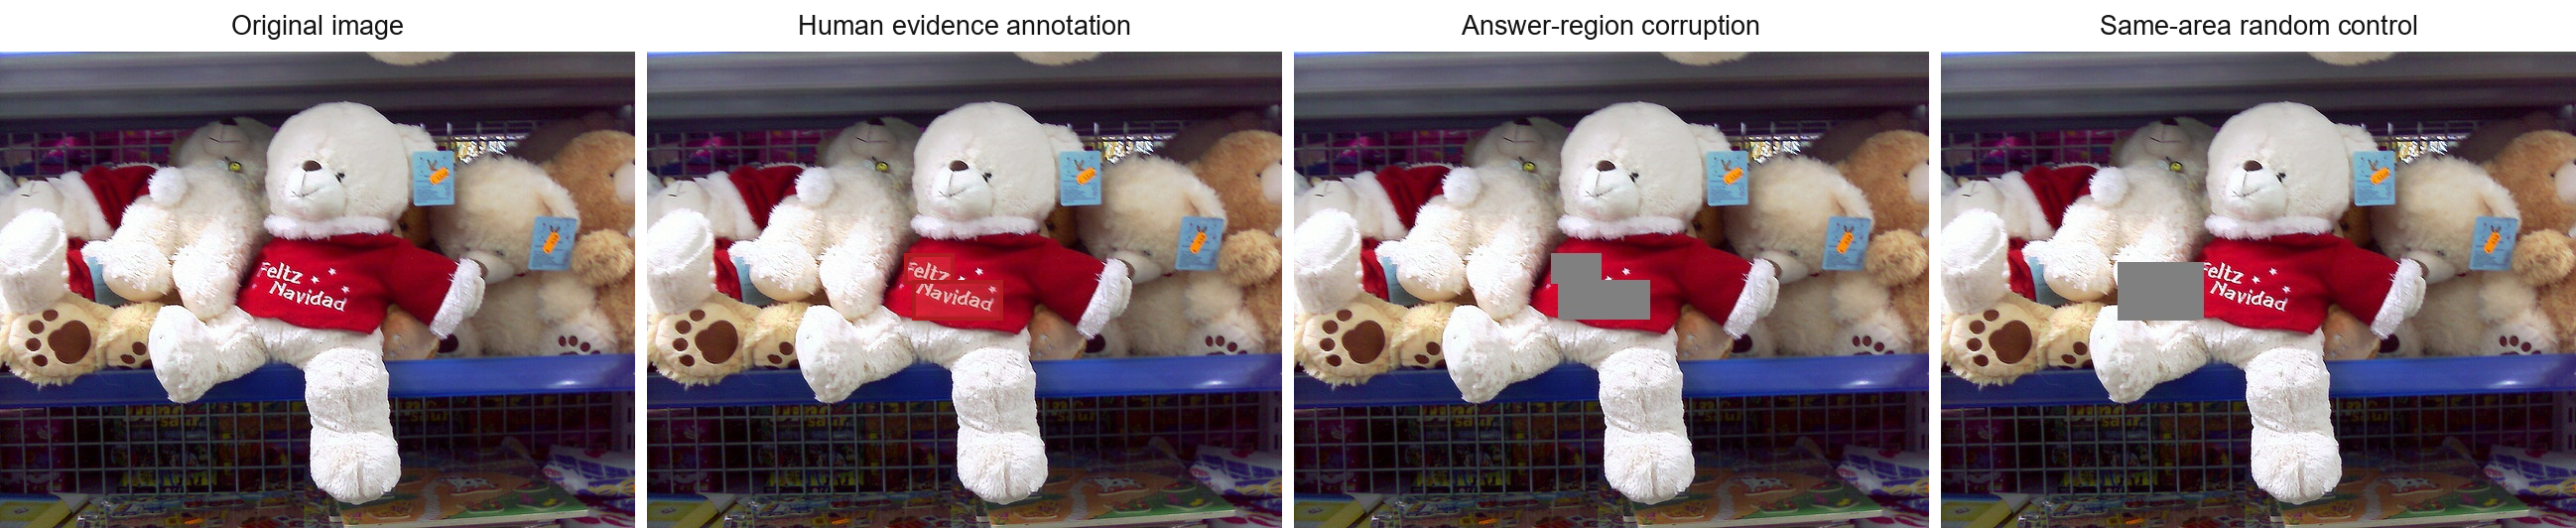
\includegraphics[width=\linewidth]{figures/okvqa_val_4739195_input_control_panel.png}
    \caption{\textbf{Example input, evidence annotation, and matched corruption.} For ``What language is the sign on the bear in?'' the target answer is ``Spanish.'' The panels show the original image, human annotation, gray answer-region corruption, and a same-area random corruption. This image illustrates mask construction; aggregate answer-score and intervention results are reported separately.}
    \label{fig:mask-annotation-example}
\end{figure}

The later full-hidden confirmation uses a different pool of 61 candidate masks. Following GPT-assisted pre-annotation, a human reviewed each mask without seeing model predictions or intervention results. One mask was rejected and the 60 accepted examples were evaluated with the interface and decision rule already frozen. This result-blind review is separate from the independently selected 52-example regional evaluation. The annotation workflow is single-pass, so no independent inter-annotator agreement estimate is available.

\section{Sparse-lens implementation and reconstruction details}
\label{app:sparse-lens-details}

The sparse analyses use frozen, model-specific PLT and CLT transcoders as post-hoc measurement interfaces; none is trained or updated on the compact-evidence evaluation samples. At read layer $\ell$, a top-$K$ reconstruction selects the $K$ largest nonnegative activations independently at each position and under each image condition, then writes their decoded sum to target layer $m$. The superscript $\ell\rightarrow m$ identifies the read and target layers, while subscript $i$ identifies the sequence position; $m=\ell$ for a PLT, whereas a CLT can use $m>\ell$. The resulting reconstruction residual is
\[
\vec{r}_{\mathrm{err},i}^{m}(x,c;\theta,\phi)
=\Delta\vec{u}_{i}^{m}(x,c;\theta)
-\widehat{\Delta\vec{u}}_{K,i}^{\ell\rightarrow m}(x,c;\theta,\phi).
\]
The decomposition experiments intervene separately with the full dense difference, its selected-feature reconstruction, and the reconstruction residual under the same answer target and mask/control setting.

The final same-object comparison uses $K\in\{16,32,64,128\}$ active features per token for all three interfaces and treats $K=128$ as the primary setting. These budgets are fixed before the 240-image confirmation results and are not selected separately for favorable answer effects. Because PLT and CLT are different fitted interfaces over different model streams, the main text compares normalized within-interface summaries rather than raw feature identities or raw cross-model effect magnitudes. Table~\ref{tab:same-object-components} reports the primary answer effects, and Table~\ref{tab:sparse-structure-summary} reports the normalized structural summaries.

The base-model identifiers are \nolinkurl{google/gemma-3-4b-it}, \nolinkurl{Qwen/Qwen2.5-VL-7B-Instruct}, and \nolinkurl{llava-hf/llava-1.5-7b-hf}. The supplementary package records these identifiers together with the lens identifiers, checkpoint hashes, layer settings, and feature metadata paths. Table~\ref{tab:sparse-lens-repro} reports the runnable settings directly. The dictionary column gives the total number of fitted sparse features; the fixed budgets select at most 16, 32, 64, or 128 active features per token. A zero in the evaluation-training column means that no evaluation row was used to fit the lens.

\begin{table}[htbp]
\centering
\small
\caption{\textbf{Sparse-tool settings for the final same-object comparison.} The layer column gives the zero-based middle language layer at which the complete feed-forward change, sparse reconstruction, and reconstruction residual are written back. No evaluation image is used to train the sparse tools.}
\label{tab:sparse-lens-repro}
\begin{tabular*}{\linewidth}{@{\extracolsep{\fill}}lcccccc@{}}
\toprule
Model & Tool & Layer & Dictionary & Budgets & Images & Evaluation training \\
\midrule
Gemma & PLT & 17 & 10,240 & 16, 32, 64, 128 & 240 & 0 \\
Qwen & PLT & 14 & 14,336 & 16, 32, 64, 128 & 240 & 0 \\
LLaVA & CLT & 16 & 16,384 & 16, 32, 64, 128 & 240 & 0 \\
\bottomrule
\end{tabular*}
\end{table}

Earlier source-tracing exports provide graph and feature-node diagnostics under different model-specific interfaces. We retain those diagnostics in the supplementary record, but they do not determine the final cross-model path conclusion. The main text instead uses the same-object sparse comparison to measure tool visibility and the native-channel experiment to test path closure without sparse-tool reconstruction error.

\section{Shared-subspace rank sweep and frozen hidden confirmation}
\label{app:shared-subspace-details}

This appendix supports Section~\ref{sec:subspace-bottleneck} by reporting the complete selection sweep at the initially selected model interfaces. Every entry is the mean restoration/corrupted-state-replacement effect as a percentage of the mean clean-minus-masked sequence-score change on the 20-example selection set. A rank would be eligible for replication only if both percentages lie between 80 and 120. None does.

\begin{center}
\captionsetup{type=table,hypcap=false}
\centering
\small
\setlength{\tabcolsep}{2.2pt}
\caption{\textbf{Complete example-shared subspace selection sweep.} Each model fits its own basis. Every cell is restoration/corrupted-state-replacement retention in percent, and Pass is 1 only when both values lie in the predeclared 80--120 interval.}
\label{tab:shared-subspace-rank-sweep}
\begin{tabular*}{\linewidth}{@{\extracolsep{\fill}}rrrrrrr@{}}
\toprule
Rank & Gemma R/D & Pass & Qwen R/D & Pass & LLaVA R/D & Pass \\
\midrule
1   & -1.3/-13.3  & 0 & -0.8/-3.1 & 0 & 0.2/1.5  & 0 \\
2   & 37.1/-32.1  & 0 & -0.4/-4.4 & 0 & 0.4/2.9  & 0 \\
4   & 23.6/-5.0   & 0 & 3.8/-1.3  & 0 & 1.8/2.0  & 0 \\
8   & 37.2/-12.5  & 0 & 2.9/-4.0  & 0 & 0.9/2.5  & 0 \\
16  & 71.0/-2.9   & 0 & 8.1/-3.9  & 0 & 5.2/6.0  & 0 \\
32  & 75.2/-2.9   & 0 & 14.6/0.8  & 0 & 7.0/2.4  & 0 \\
64  & 102.6/-14.1 & 0 & 45.2/11.8 & 0 & 11.2/4.4 & 0 \\
128 & 120.7/-20.6 & 0 & 51.7/22.6 & 0 & 21.0/7.5 & 0 \\
\bottomrule
\end{tabular*}
\end{center}

The fitting, selection, and replication images are disjoint within this experiment. The basis is fitted only on the 40 fitting images, and the candidate rank is chosen only from the 20 selection images. Because no rank passes selection, the 40-image replication summaries in Table~\ref{tab:shared-subspace-summary} are diagnostic rather than a strict confirmation of any selected rank.

The full-hidden reference uses the same initial frozen model interfaces without projection. Only the evaluated LLaVA interface has restoration and corrupted-state-replacement means inside the target interval on both selection and replication. Its separate 60-example confirmation uses a frozen manifest produced after result-blind human mask review. The review accepts 60 of 61 candidates, requires no mask corrections, and excludes the rejected example before model evaluation. The interface, decision rule, and sample manifest are unchanged during that confirmation run.

The follow-up repeats the rank sweep at each model's penultimate language layer and four answer-adjacent positions, using the same 40 fitting, 20 selection, and 40 replication image IDs in all three models. Table~\ref{tab:matched-late-subspace} gives every rank's two selection-set means. No candidate reaches the 80--120\% interval in both directions. The relative-layer rule was added after the earlier LLaVA observation and is a matched diagnostic, not a second jointly prospective confirmation.

\begin{samepage}
\begin{center}
\begin{minipage}{\linewidth}
\captionsetup{type=table,hypcap=false}
\caption{\textbf{No shared low-rank projection passes at the matched late-answer interfaces.} Each model fits its own basis on the same 40 images and evaluates the same 20 selection images at its penultimate language layer and four answer-adjacent positions. Cells show restoration/corrupted-state-replacement as percentages of that model's mean clean-minus-masked sequence-score change. A rank advances only if both means lie in 80--120\%; all 24 candidate-model combinations fail. The 40-image replication split is retained for diagnostic summaries, not for strict confirmation of a selected rank.}
\label{tab:matched-late-subspace}
\centering
\normalsize
\setlength{\tabcolsep}{3pt}
\begin{tabular*}{\linewidth}{@{\extracolsep{\fill}}rrrr@{}}
\toprule
Rank & Gemma R/C & Qwen R/C & LLaVA R/C \\
\midrule
1 & -43.2/-17.4 & -6.2/-4.9 & 1.5/1.6 \\
2 & -38.2/-15.3 & -5.5/-5.6 & 1.2/1.7 \\
4 & -35.4/-17.6 & -6.3/-6.1 & 3.0/2.4 \\
8 & -45.0/-27.3 & -4.0/-5.4 & 2.0/4.2 \\
16 & -48.5/-23.1 & 14.7/0.0 & 6.7/5.0 \\
32 & -40.8/-25.6 & 19.0/-6.1 & 8.3/4.6 \\
64 & -28.0/-19.7 & 21.1/-3.5 & 11.0/6.0 \\
128 & -19.3/-12.9 & 25.3/-3.6 & 23.7/12.6 \\
\bottomrule
\end{tabular*}
\end{minipage}
\end{center}
\end{samepage}


The unprojected full-hidden reference is reported separately from the selected low-rank candidates. In the follow-up's 20-image selection split, Gemma restores/replaces 86.6\%/85.1\% of its mean clean-minus-masked sequence-score change, Qwen 88.0\%/68.3\%, and LLaVA 93.4\%/90.9\%. Gemma does not retain that mean match on the 40-image replication split: its mean clean-minus-masked sequence-score change is only $0.0184$, while restoration and corrupted-state replacement change the score by $0.3904$ and $0.3708$. Ratios to this near-zero reference are unstable and are not interpreted. On the same replication split, Qwen's replacement remains below the lower gate; LLaVA's unprojected interface passes all four paired bootstrap bounds. These reused splits complement, but do not replace, the separate 60-example LLaVA confirmation.

\section{Additional controls for localized visual evidence}
\label{app:regional-controls}

The main input comparison contrasts answer-region corruption with same-area random corruption on the same image. Additional operators test whether the rank pattern depends on one gray-mask implementation. Table~\ref{tab:stronger-mask-controls} reports target-rank damage relative to the clean image; larger values indicate a larger loss of target support. The expanded answer entry ranges over gray, blur, inpainting, and patch-shuffle corruptions, whereas the random entry uses a same-area region. The independently selected columns summarize the separate 52-example gray-mask comparison. These controls support the regional answer-score finding rather than the internal path result.

\begin{table}[htbp]
\centering
\normalsize
\caption{\textbf{Answer-region versus matched-random rank damage.} Expanded answer entries give the range across four answer-region operators; other entries are mean damage for the named condition. Values are interpreted within model because target-rank scales differ.}
\label{tab:stronger-mask-controls}
\begin{tabular*}{\linewidth}{@{\extracolsep{\fill}}lrrrr@{}}
\toprule
Model & Expanded answer & Expanded random & Independent answer & Independent random \\
\midrule
Gemma & $9613$--$16342$ & $951$ & $5028$ & $-120$ \\
Qwen & $2795$--$3131$ & $50$ & $297$ & $-39$ \\
LLaVA & $73$--$98$ & $-2.5$ & $46$ & $0$ \\
\bottomrule
\end{tabular*}
\end{table}

Mask morphology supplies a complementary localized check. Dilation and erosion preserve the direction of the earlier Gemma hidden-state diagnostic and Qwen sparse-feature diagnostic. These model-specific checks address sensitivity to one exact polygon boundary; the shared three-model, same-area comparison remains the primary regional control.

\section{Prompt wording and question-paraphrase robustness}
\label{app:prompt-text}

All prompt families append the same answer format, ``\texttt{The answer is <short answer>},'' to the original or paraphrased question. They differ only in whether they add no cue (\texttt{B\_direct}), internal step-by-step reasoning (\texttt{C\_step\_only}), visual evidence (\texttt{D\_visual\_only}), or both reasoning and visual evidence (\texttt{A\_step\_visual}). Some main analyses use only the \texttt{B\_direct} and \texttt{D\_visual\_only} subset, while this diagnostic uses all four families.

The wording and question-paraphrase grid tests whether the evidence-to-answer effect is merely driven by wording. These analyses predate the final same-object sparse comparison and are retained as auxiliary identity and hidden-state diagnostics. The unified \modelgemma{} and \modelqwen{} analysis separates fixed-node strength from route-identity stability. Table~\ref{tab:wording-grid} summarizes the diagnostic counts and model-appropriate stability statistics. For Gemma, the two counts are fixed-node rows and target-aligned rows; for Qwen, they are candidate-metric rows and top-$K$ overlap rows; for LLaVA, they are evaluated condition keys and image--question samples. Node or feature overlap compares sparse identities, structural overlap compares Gemma graph edges or Qwen layer--position--feature identities, and the hidden positive fraction is the proportion of LLaVA condition keys with a positive hidden-restoration logit effect. NA denotes an unavailable quantity, not a zero effect. Route identity is only moderately stable, so these diagnostics do not establish fixed-node invariance or positive causal coverage by the fitted sparse tools.

\begin{table}[htbp]
\centering
\small
\caption{\textbf{Wording diagnostic matrix.} Counts use the row-specific units defined in the preceding text. Sparse-overlap columns apply to Gemma and Qwen; the hidden positive fraction applies to LLaVA.}
\label{tab:wording-grid}
\begin{tabular*}{\linewidth}{@{\extracolsep{\fill}}lrrrrr@{}}
\toprule
Analysis & \shortstack{Full\\count} & \shortstack{Analysis\\count} & \shortstack{Node/feature\\overlap} & \shortstack{Structural\\overlap} & \shortstack{Hidden positive\\fraction} \\
\midrule
Gemma graph & 524 & 414 & 0.280 & 0.183 & NA \\
Qwen route rediscovery & 4608 & 576 & 0.596 & 0.409 & NA \\
LLaVA hidden grid & 576 & 12 & NA & NA & 0.852 \\
\bottomrule
\end{tabular*}
\end{table}

Changing the question wording or prompt family can therefore change \emph{which sparse identities or hidden-effect pattern is observed}, even when the image evidence and answer remain the same. This observation establishes measurement sensitivity to wording; it does not by itself identify a different native computation. We therefore avoid claiming fixed-node invariance across prompts.

The LLaVA wording grid provides a hidden-level robustness check rather than a grouped-route identity test. Its hidden-logit positive fraction is $0.852$ overall and ranges from $0.833$ to $0.891$ across the reported prompt-family and question-variant summaries. Wording changes therefore modulate effect size without removing the hidden-level intervention signal.

\begin{figure}[htbp]
    \centering
    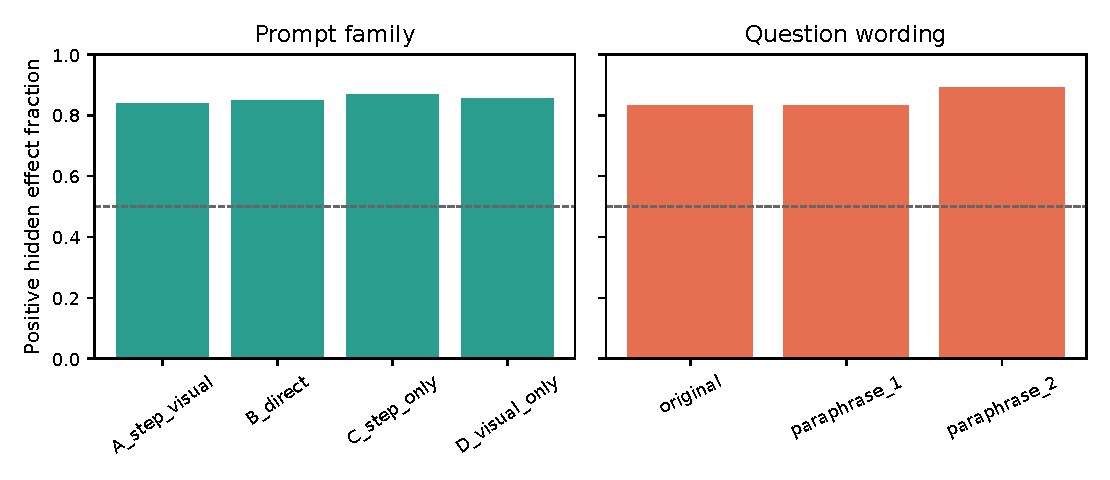
\includegraphics[width=0.88\linewidth]{figures/llava_prompt_text_grid.pdf}
    \caption{\textbf{LLaVA prompt and question-variant grid.} Cells summarize hidden-level effect direction across prompt families and paraphrases.}
    \label{fig:prompt-grid}
\end{figure}

Together, these diagnostics support a careful secondary conclusion: prompt and wording changes modulate observable sparse identity and hidden-effect allocation, but do not explain away the hidden-state evidence-to-answer dependence measured by the final intervention tests.

\FloatBarrier


\end{document}
